%% bare_conf_compsoc.tex
%% V1.4b
%% 2015/08/26
%% by Michael Shell
%% See:
%% http://www.michaelshell.org/
%% for current contact information.
%%
%% This is a skeleton file demonstrating the use of IEEEtran.cls
%% (requires IEEEtran.cls version 1.8b or later) with an IEEE Computer
%% Society conference paper.
%%
%% Support sites:
%% http://www.michaelshell.org/tex/ieeetran/
%% http://www.ctan.org/pkg/ieeetran
%% and
%% http://www.ieee.org/

\documentclass[conference,compsoc]{IEEEtran}
% Some/most Computer Society conferences require the compsoc mode option,
% but others may want the standard conference format.
%
% If IEEEtran.cls has not been installed into the LaTeX system files,
% manually specify the path to it like:
% \documentclass[conference,compsoc]{../sty/IEEEtran}

% *** MISC UTILITY PACKAGES ***
%
\usepackage{ifpdf}
\usepackage{framed}
% Heiko Oberdiek's ifpdf.sty is very useful if you need conditional
% compilation based on whether the output is pdf or dvi.
% usage:
% \ifpdf
%   % pdf code
% \else
%   % dvi code
% \fi
% The latest version of ifpdf.sty can be obtained from:
% http://www.ctan.org/pkg/ifpdf
% Also, note that IEEEtran.cls V1.7 and later provides a builtin
% \ifCLASSINFOpdf conditional that works the same way.
% When switching from latex to pdflatex and vice-versa, the compiler may
% have to be run twice to clear warning/error messages.



% *** CITATION PACKAGES ***
%
\ifCLASSOPTIONcompsoc
  % IEEE Computer Society needs nocompress option
  % requires cite.sty v4.0 or later (November 2003)
  \usepackage[nocompress]{cite}
\else
  % normal IEEE
  \usepackage{cite}
\fi



% *** GRAPHICS RELATED PACKAGES ***
%
\ifCLASSINFOpdf
  % \usepackage[pdftex]{graphicx}
  % declare the path(s) where your graphic files are
  % \graphicspath{{../pdf/}{../jpeg/}}
  % and their extensions so you won't have to specify these with
  % every instance of \includegraphics
  % \DeclareGraphicsExtensions{.pdf,.jpeg,.png}
\else
  % or other class option (dvipsone, dvipdf, if not using dvips). graphicx
  % will default to the driver specified in the system graphics.cfg if no
  % driver is specified.
  % \usepackage[dvips]{graphicx}
  % declare the path(s) where your graphic files are
  % \graphicspath{{../eps/}}
  % and their extensions so you won't have to specify these with
  % every instance of \includegraphics
  % \DeclareGraphicsExtensions{.eps}
\fi
% graphicx was written by David Carlisle and Sebastian Rahtz. It is
% required if you want graphics, photos, etc. graphicx.sty is already
% installed on most LaTeX systems. The latest version and documentation
% can be obtained at: 
% http://www.ctan.org/pkg/graphicx
% Another good source of documentation is "Using Imported Graphics in
% LaTeX2e" by Keith Reckdahl which can be found at:
% http://www.ctan.org/pkg/epslatex
%
% latex, and pdflatex in dvi mode, support graphics in encapsulated
% postscript (.eps) format. pdflatex in pdf mode supports graphics
% in .pdf, .jpeg, .png and .mps (metapost) formats. Users should ensure
% that all non-photo figures use a vector format (.eps, .pdf, .mps) and
% not a bitmapped formats (.jpeg, .png). The IEEE frowns on bitmapped formats
% which can result in "jaggedy"/blurry rendering of lines and letters as
% well as large increases in file sizes.
%
% You can find documentation about the pdfTeX application at:
% http://www.tug.org/applications/pdftex





% *** MATH PACKAGES ***
%
\usepackage{amsmath}
\usepackage{cuted}
% A popular package from the American Mathematical Society that provides
% many useful and powerful commands for dealing with mathematics.
%
% Note that the amsmath package sets \interdisplaylinepenalty to 10000
% thus preventing page breaks from occurring within multiline equations. Use:
%\interdisplaylinepenalty=2500
% after loading amsmath to restore such page breaks as IEEEtran.cls normally
% does. amsmath.sty is already installed on most LaTeX systems. The latest
% version and documentation can be obtained at:
% http://www.ctan.org/pkg/amsmath
\newcommand\numberthis{\addtocounter{equation}{1}\tag{\theequation}}




% *** SPECIALIZED LIST PACKAGES ***
%
\usepackage{algorithmic}
% algorithmic.sty was written by Peter Williams and Rogerio Brito.
% This package provides an algorithmic environment fo describing algorithms.
% You can use the algorithmic environment in-text or within a figure
% environment to provide for a floating algorithm. Do NOT use the algorithm
% floating environment provided by algorithm.sty (by the same authors) or
% algorithm2e.sty (by Christophe Fiorio) as the IEEE does not use dedicated
% algorithm float types and packages that provide these will not provide
% correct IEEE style captions. The latest version and documentation of
% algorithmic.sty can be obtained at:
% http://www.ctan.org/pkg/algorithms
% Also of interest may be the (relatively newer and more customizable)
% algorithmicx.sty package by Szasz Janos:
% http://www.ctan.org/pkg/algorithmicx




% *** ALIGNMENT PACKAGES ***
%
\usepackage{array}
% Frank Mittelbach's and David Carlisle's array.sty patches and improves
% the standard LaTeX2e array and tabular environments to provide better
% appearance and additional user controls. As the default LaTeX2e table
% generation code is lacking to the point of almost being broken with
% respect to the quality of the end results, all users are strongly
% advised to use an enhanced (at the very least that provided by array.sty)
% set of table tools. array.sty is already installed on most systems. The
% latest version and documentation can be obtained at:
% http://www.ctan.org/pkg/array


% IEEEtran contains the IEEEeqnarray family of commands that can be used to
% generate multiline equations as well as matrices, tables, etc., of high
% quality.




% *** SUBFIGURE PACKAGES ***
%\ifCLASSOPTIONcompsoc
%  \usepackage[caption=false,font=footnotesize,labelfont=sf,textfont=sf]{subfig}
%\else
%  \usepackage[caption=false,font=footnotesize]{subfig}
%\fi
% subfig.sty, written by Steven Douglas Cochran, is the modern replacement
% for subfigure.sty, the latter of which is no longer maintained and is
% incompatible with some LaTeX packages including fixltx2e. However,
% subfig.sty requires and automatically loads Axel Sommerfeldt's caption.sty
% which will override IEEEtran.cls' handling of captions and this will result
% in non-IEEE style figure/table captions. To prevent this problem, be sure
% and invoke subfig.sty's "caption=false" package option (available since
% subfig.sty version 1.3, 2005/06/28) as this is will preserve IEEEtran.cls
% handling of captions.
% Note that the Computer Society format requires a sans serif font rather
% than the serif font used in traditional IEEE formatting and thus the need
% to invoke different subfig.sty package options depending on whether
% compsoc mode has been enabled.
%
% The latest version and documentation of subfig.sty can be obtained at:
% http://www.ctan.org/pkg/subfig
\usepackage{verbatim}
\usepackage{soul}
\usepackage{xcolor}
\newcommand{\TODO}[1]{\hl{TODO: #1}}
\newcommand{\NOTE}[1]{\hl {NOTE: #1}}
\newcommand{\changed}[1]{\textcolor{red}{#1}}


% *** FLOAT PACKAGES ***
%
%\usepackage{fixltx2e}
% fixltx2e, the successor to the earlier fix2col.sty, was written by
% Frank Mittelbach and David Carlisle. This package corrects a few problems
% in the LaTeX2e kernel, the most notable of which is that in current
% LaTeX2e releases, the ordering of single and double column floats is not
% guaranteed to be preserved. Thus, an unpatched LaTeX2e can allow a
% single column figure to be placed prior to an earlier double column
% figure.
% Be aware that LaTeX2e kernels dated 2015 and later have fixltx2e.sty's
% corrections already built into the system in which case a warning will
% be issued if an attempt is made to load fixltx2e.sty as it is no longer
% needed.
% The latest version and documentation can be found at:
% http://www.ctan.org/pkg/fixltx2e


%\usepackage{stfloats}
% stfloats.sty was written by Sigitas Tolusis. This package gives LaTeX2e
% the ability to do double column floats at the bottom of the page as well
% as the top. (e.g., "\begin{figure*}[!b]" is not normally possible in
% LaTeX2e). It also provides a command:
%\fnbelowfloat
% to enable the placement of footnotes below bottom floats (the standard
% LaTeX2e kernel puts them above bottom floats). This is an invasive package
% which rewrites many portions of the LaTeX2e float routines. It may not work
% with other packages that modify the LaTeX2e float routines. The latest
% version and documentation can be obtained at:
% http://www.ctan.org/pkg/stfloats
% Do not use the stfloats baselinefloat ability as the IEEE does not allow
% \baselineskip to stretch. Authors submitting work to the IEEE should note
% that the IEEE rarely uses double column equations and that authors should try
% to avoid such use. Do not be tempted to use the cuted.sty or midfloat.sty
% packages (also by Sigitas Tolusis) as the IEEE does not format its papers in
% such ways.
% Do not attempt to use stfloats with fixltx2e as they are incompatible.
% Instead, use Morten Hogholm'a dblfloatfix which combines the features
% of both fixltx2e and stfloats:
%
% \usepackage{dblfloatfix}
% The latest version can be found at:
% http://www.ctan.org/pkg/dblfloatfix




% *** PDF, URL AND HYPERLINK PACKAGES ***
%
\usepackage{url}
% url.sty was written by Donald Arseneau. It provides better support for
% handling and breaking URLs. url.sty is already installed on most LaTeX
% systems. The latest version and documentation can be obtained at:
% http://www.ctan.org/pkg/url
% Basically, \url{my_url_here}.

\usepackage{graphicx} % Required for including pictures
\graphicspath{{pics/}} % Specifies the directory where pictures are stored
\usepackage{caption}
\usepackage{subcaption}
\usepackage{booktabs}
\usepackage{multirow} % make table

\makeatletter % Put Roman Number in Text
\newcommand{\rmnum}[1]{\romannumeral #1}
\newcommand{\Rmnum}[1]{\expandafter\@slowromancap\romannumeral #1@}
\makeatother



% *** Do not adjust lengths that control margins, column widths, etc. ***
% *** Do not use packages that alter fonts (such as pslatex).         ***
% There should be no need to do such things with IEEEtran.cls V1.6 and later.
% (Unless specifically asked to do so by the journal or conference you plan
% to submit to, of course. )


% correct bad hyphenation here
\hyphenation{op-tical net-works semi-conduc-tor}


\begin{document}
%
% paper title
% Titles are generally capitalized except for words such as a, an, and, as,
% at, but, by, for, in, nor, of, on, or, the, to and up, which are usually
% not capitalized unless they are the first or last word of the title.
% Linebreaks \\ can be used within to get better formatting as desired.
% Do not put math or special symbols in the title.
\title{Watch Out for the Bully! Job Interference Study on Dragonfly Network}


% author names and affiliations
% use a multiple column layout for up to three different
% affiliations
% \author{\IEEEauthorblockN{Michael Shell}
% \IEEEauthorblockA{School of Electrical and\\Computer Engineering\\
% Georgia Institute of Technology\\
% Atlanta, Georgia 30332--0250\\
% Email: http://www.michaelshell.org/contact.html}
% \and
% \IEEEauthorblockN{Homer Simpson}
% \IEEEauthorblockA{Twentieth Century Fox\\
% Springfield, USA\\
% Email: homer@thesimpsons.com}
% \and
% \IEEEauthorblockN{James Kirk\\ and Montgomery Scott}
% \IEEEauthorblockA{Starfleet Academy\\
% San Francisco, California 96678-2391\\
% Telephone: (800) 555--1212\\
% Fax: (888) 555--1212}}


\author{

\IEEEauthorblockN{Xu Yang\IEEEauthorrefmark{1}, John Jenkins\IEEEauthorrefmark{2}, Misbah Mubarak\IEEEauthorrefmark{2}, Robert B. Ross\IEEEauthorrefmark{2}, Zhiling Lan\IEEEauthorrefmark{1}}

\IEEEauthorblockA{\IEEEauthorrefmark{1}Department of Computer Science,
Illinois Institute of Technology,
Chicago, Illinois, USA 60616\\
\{xyang56\}@hawk.iit.edu, lan@iit.edu}

\IEEEauthorblockA{\IEEEauthorrefmark{2}Mathematics and Computer Science Division, Argonne National Laboratory,
Argonne, IL, USA 60439\\
\{jenkins,rross\}@mcs.anl.gov, mmubarak@anl.gov}
}


% conference papers do not typically use \thanks and this command
% is locked out in conference mode. If really needed, such as for
% the acknowledgment of grants, issue a \IEEEoverridecommandlockouts
% after \documentclass

% for over three affiliations, or if they all won't fit within the width
% of the page (and note that there is less available width in this regard for
% compsoc conferences compared to traditional conferences), use this
% alternative format:
% 
%\author{\IEEEauthorblockN{Michael Shell\IEEEauthorrefmark{1},
%Homer Simpson\IEEEauthorrefmark{2},
%James Kirk\IEEEauthorrefmark{3}, 
%Montgomery Scott\IEEEauthorrefmark{3} and
%Eldon Tyrell\IEEEauthorrefmark{4}}
%\IEEEauthorblockA{\IEEEauthorrefmark{1}School of Electrical and Computer Engineering\\
%Georgia Institute of Technology,
%Atlanta, Georgia 30332--0250\\ Email: see http://www.michaelshell.org/contact.html}
%\IEEEauthorblockA{\IEEEauthorrefmark{2}Twentieth Century Fox, Springfield, USA\\
%Email: homer@thesimpsons.com}
%\IEEEauthorblockA{\IEEEauthorrefmark{3}Starfleet Academy, San Francisco, California 96678-2391\\
%Telephone: (800) 555--1212, Fax: (888) 555--1212}
%\IEEEauthorblockA{\IEEEauthorrefmark{4}Tyrell Inc., 123 Replicant Street, Los Angeles, California 90210--4321}}




% use for special paper notices
%\IEEEspecialpapernotice{(Invited Paper)}




% make the title area
\maketitle

% As a general rule, do not put math, special symbols or citations
% in the abstract
\begin{abstract}

The high-radix, low-diameter dragonfly network will be the choice of many computing facilities for building their next generation supercomputers. Preliminary studies show that random placement with adaptive routing should be the rule of thumb to utilize such networks, since random placement with adaptive routing can uniformly distribute traffic over the network and alleviate congestion. However, in this paper, we made the observation that while random placement coupled with adaptive routing can load-balance the network when multiple jobs are running concurrently, they can not guarantee the best performance for each single job. The performance improvement of communication-intensive jobs comes with the sacrifice of less intensive jobs. We refer this phenomenon as ``bully" between concurrently running jobs. We presented a detailed analysis about this ``bully" behavior between jobs at the network level based on a sophisticated, high-fidelity discrete even-driven simulation tool. The observations and analysis presented in this work illuminate a path to the adoption of more efficient job placement policy and routing algorithm for HPC systems with dragonfly network.  

\end{abstract}

% no keywords

% \keywords{Dragonfly, Job placement, Routing, Interference}



% For peer review papers, you can put extra information on the cover
% page as needed:
% \ifCLASSOPTIONpeerreview
% \begin{center} \bfseries EDICS Category: 3-BBND \end{center}
% \fi
%
% For peerreview papers, this IEEEtran command inserts a page break and
% creates the second title. It will be ignored for other modes.
\IEEEpeerreviewmaketitle



\section{Introduction}
\label{sec:intro}

The low latency and high bandwidth interconnect network plays a critical role in HPC system performance. As computational capabilities continue to grow due to many-core nodes with accelerators, the network is increasingly becoming a scarce resource. The high-radix, low-diameter dragonfly topology can lower the extension cost of the interconnect, improve network bandwidth and reduce packet latency \cite{dally-dragonfly}. This make the dragonfly network a very promising choice for building petaflop and beyond supercomputers. 
%The procurement results from Trinity and CORAL project shows the great performance improvement can be got from using dragonfly network. 


While dragonfly topologies provide low-latency and high-bandwidth networking, efficiently utilizing it is a significant concern. In particular, intelligent job placement to avoid interference is of paramount importance to guarantee the performance of each job when it shares network resources with other concurrently running peers \cite{bhatele2015, dskinner}. Recent studies suggest that random job placement coupled with adaptive routing can alleviate local congestion, eliminate hot-spots and reach load-balance for dragonfly networks \cite{jain-sc14, bhatele-sc11, brandt2014}. 


In this work, we study the interference between concurrently running jobs on dragonfly networks with different job placement and routing policies. We use CODES, an HPC network simulation toolkit with high fidelity and excellent scalability for packet level simulation \cite{codes}. Unlike much existing work that rely on synthetic workloads, we use traces of three representative applications from the DOE Design Forward Project \cite{designforwardwebpage}. The advantage of using real application traces is straight forward: these traces can capture detailed application communication behaviors that are  omitted in synthetic workload for simplification. Applications are usually distinctive from each other in data transfer amount, communication pattern, operation dependency etc., which can be impractical to reproduce in a synthetic workload.

We conduct extensive experiments with three applications running on dragonfly network with two job placement policies and three routing policies. We analyze the performance of network as well as individual application when running with different placement and routing configurations. Our evaluation is based on more than 1000 runs of simulation. We make the following interesting observations through extensive simulation.


\begin{itemize}
   
    \item Random placement coupled with adaptive routing can uniformly distribute traffic over the network, avoid hot-spots and alleviate traffic congestion, optimizing the overall performance of the dragonfly network. 
    
    \item The ``bully" behavior occurs between concurrently running jobs on a dragonfly network when random placement and adaptive routing are in use. Communication-intensive jobs obtain performance improvement at the expense of less intensive jobs suffering performance degradation. 
    
    \item Random placement coupled with adaptive routing can improve the performance of communication-intensive jobs by enabling network resource sharing, though it introduces interference between concurrently running jobs.
    
    \item Contiguous placement coupled with minimal routing can guarantee consistency performance of less communication-intensive jobs by prohibiting network resource sharing, though it results in local network congestion and unbalanced network utilization.
    
\end{itemize}

Based on our observations, the optimal job placement and routing solution for the workload running dragonfly system should be specific to the job communication intensity. \emph{The random placement and adaptive routing are preferable to communication-intensive jobs, whereas contiguous placement and minimal routing are in favor of less intensive jobs.} To the best of our knowledge, using parallel application traces from production systems for the study of job interference on dragonfly networks has not been reported so far. We believe the observations and analysis presented in this paper are valuable to a number of communities including HPC computing centers, system software developers, and system administrators. For example, the computing centers should take resource sharing into consideration when choosing proper configurations for building their dragonfly networks. System software developers could design better scheduling algorithms for jobs with distinct communication behavior. System administrators could make more accurate predication about system availability based on job running status under different placement and routing configurations.

The rest of this paper is organized as follows. Section \ref{sec:background} describes an implementation of the dragonfly network, introduces the placement policies and routing policies. Section \ref{sec: methodology} talks about the use of CODES as a research vehicle and three representative applications from the DOE Design Forward Project. Section \ref{sec:workload-1} presents the observations and analysis of three applications running on a dragonfly network with different placement and routing configurations. Section \ref{sec:workload-2} validates the observations we obtain from previous section. Section \ref{sec: hybrid placement} presents a alternative placement policy for the dragonfly network. Section \ref{sec:related work} discusses the related work. Finally, the conclusion is presented in Section \ref{sec:conclusion}.

\section{Background}
\label{sec:background}

In this section, we review the dragonfly topology, including the placement and routing policies examined in previous work. 

\subsection{Dragonfly Network}
\label{sec:network}
The dragonfly is a two-level hierarchical topology, consisting of several groups connected by all-to-all links. In each group, there could be $a$ routers connected via all-to-all local channels. For each router, there could be $p$ compute nodes attached to it via terminal links. The router has $h$ global channels used as intergroup connections through which the router connected to other routers in different groups. Thus, the radix of each router is $k = a+h+p-1$. Different computing centers could choose different values for  $a$, $h$, $p$ when deploying their dragonfly network. The adoption of proper $a$, $h$, $p$ involves many factors, such as system scale, building cost and workload. 

It is recommended that for the load balance purpose, a proper dragonfly configuration should follow $a=2p=2h$~\cite{kim-micro}. Under this configuration, the total number of groups, denoted as $g$ in the dragonfly network would be $g = a*h+1 $, the total number of compute nodes denoted as $N$ in the network would be $N = p*a*g $. An implementation of dragonfly network follows such configuration is illustrated in Figure~\ref{fig:dragonfly-overview}. There are six routers in each group, each router has three compute nodes attached to it. This dragonfly network consists of 19 groups and 342 nodes in total.

\begin{figure}[h!] 
  \centering
  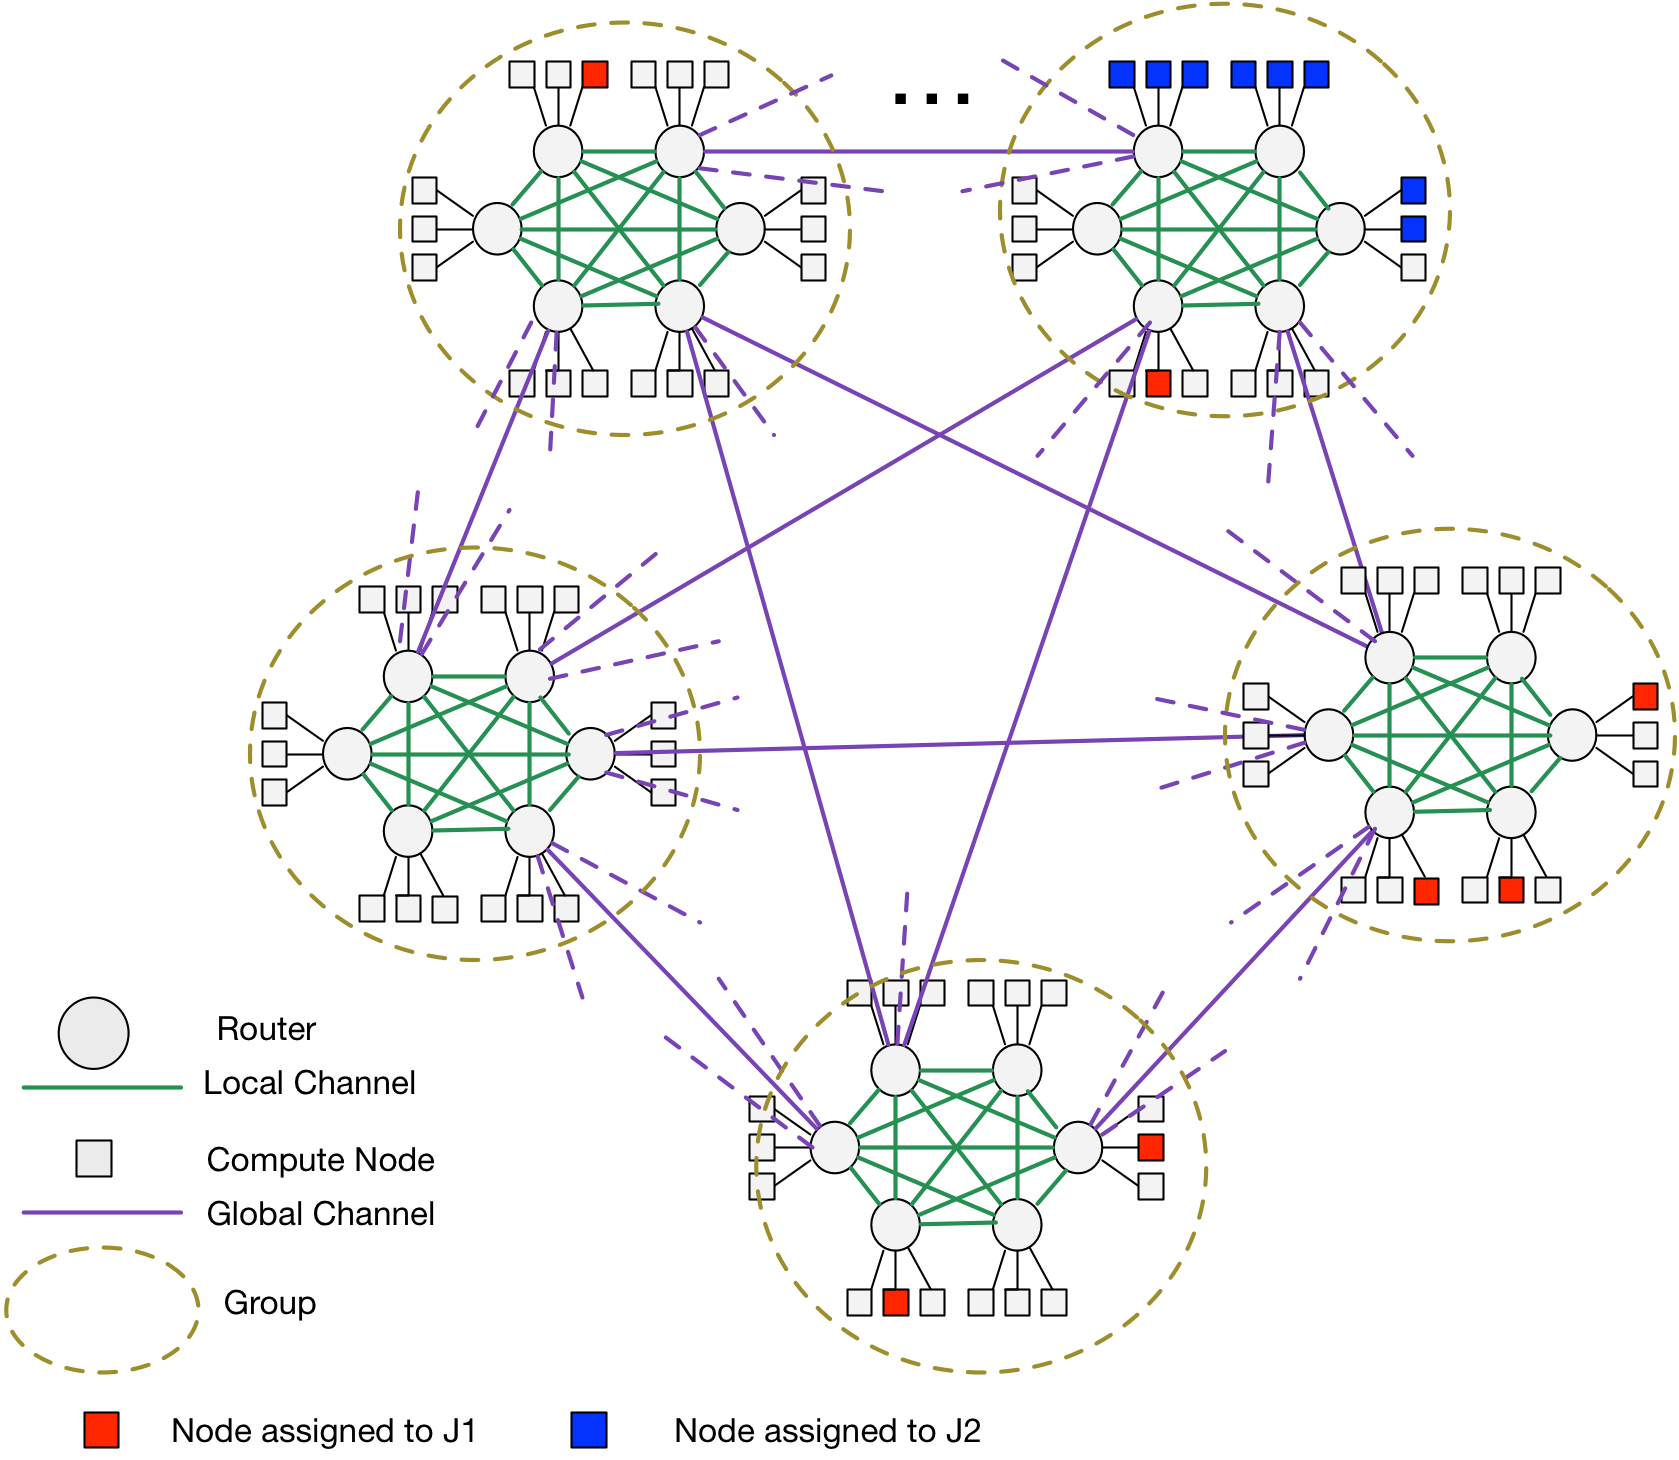
\includegraphics[width=0.48\textwidth]{dragonfly-overview}
  \caption{Dragonfly Network Overview. There are 19 groups, six routers in each group, three compute nodes connected to each router, 342 nodes in total. Job $J1$ requires seven nodes, getting its allocation by random placement. Job $J2$ requires eight nodes, getting its allocation by contiguous placement.}
  \label{fig:dragonfly-overview}
\end{figure}


\subsection{Job Placement on Dragonfly}
\label{sec:placement-schemes}

For a parallel application requiring multiple compute nodes, job placement policy refers to the way of assigning tasks of the application onto the system by a system software such as batch scheduler~\cite{xu-cluster14}. In this work, we study two alternative placement policies considered by the community for dragonfly systems: 


\textbf{Contiguous Placement:} In this policy, the compute nodes are assigned to a job in a consecutive manner. The assignment first fills up a group, then crosses group boundaries and starts to fill the next group if necessary. As shown in Figure~\ref{fig:dragonfly-overview}, $J2$ gets eight nodes by contiguous placement. Contiguous placement confines the tasks of a job into the same group, which may result in local network congestion and increase the possibility of hot-spots. 

\textbf{Random Placement:} In this policy, a job gets a set of nodes randomly selected from all the available nodes in the system. The nodes assigned to $J1$ in Figure~\ref{fig:dragonfly-overview} are attached to different routers in different groups. Routers may be shared by different jobs when random placement is in use. Random placement can distribute the tasks of a job uniformly across the whole system to avoid the possible local congestion. However, random placement may cause possible congestion on global links.


\subsection{Routing on Dragonfly}
\label{sec:routing-schemes}

The routing policy refers to the strategy adopted to route a message (a stream of packets) from the source router to the destination router. Previously studied routing policies for dragonfly network include minimal routing, adaptive routing~\cite{dally-dragonfly}, progressive adaptive routing~\cite{jiang} and some of their variations~\cite{won-prog-adaptive}. In this work we study three widely adopted routing policies on dragonfly networks.

\textbf{Minimal:} In this policy, a message takes the shortest path from the source router to the destination router. When there are multiple shortest paths between the source and destination router, the message will be evenly divided among the paths. Minimal routing can guarantee the minimum hops the message takes from source to destination. However, it may result in congestion along the shortest path. 

\textbf{Adaptive:} In this policy, the path a message takes will be adaptively chosen between shortest and non-shortest paths, depending on the congestion situation along those paths. For the non-shortest path, an intermediate router will be randomly chosen. The message takes the intermediate router as a via point, connecting the source and destination router through two separate shortest paths. Adaptive routing can avoid hot-spots in the presence of congestion and collapse to minimal routing otherwise. 

\textbf{Progressive Adaptive:} In this policy, the decision to route minimally at each hop in the source group will be re-evaluated. Any decision to route non-minimally at source router or at a subsequent hop is permanent and will not be re-evaluated~\cite{jiang}. The progressive adaptive is capable of handling the case where a global channel is congested but the source router has not been informed yet~\cite{jiang}. The packet will take the non-minimal route only when the congestion is encountered. 



\section{Methodology}
\label{sec: methodology}

It is difficult to experiment with concurrently running jobs on HPC system~\cite{zhou-ipdps-2015}\cite{jain-sc14}\cite{bhatele-sc11}\cite{jokanovic-ipdps-2015}. One reason is that job placement and routing policies are part of system configuration, which is impossible for user to make changes at will. Another reason is that it is unrealistic to reserve the system exclusively to run the same batch of jobs with desired placement and routing configurations and compare the results. The third reason is that configurable dragonfly networks that allow us to perform the exploration presented in this paper are hard to come by for the time being. Therefore, we resort to simulation in our work.

\subsection{Simulation Tool}
\label{sec:simulation-tool}

A simulation toolkit named CODES, Co-Design of Multilayer Exascale Storage Architectures, enables the exploration of simulating different HPC networks with high fidelity and great scalability~\cite{codes}. CODES supports dragonfly~\cite{codes-dragonfly}~\cite{misbah-tpds}, torus~\cite{misbah-pads-2014}~\cite{ning-pads-2011}, and fat-tree~\cite{ning-pads-2015} networks with packet-level high-fidelity simulation. It can drive these models through an MPI simulation layer utilizing DUMPI traces~\cite{sst}. In this work, we perform an in-depth analysis of network performance as well as job interference when different job placement and routing policies are in use on the dragonfly network.

\subsection{Parallel Applications}
\label{sec: application traces}

We choose three parallel applications from the DOE Design Forward Project~\cite{designforwardwebpage}, which can represent of a wide array of applications running on leadership-class supercomputers. Specifically, we study the \emph{Algebraic MultiGrid Solver} (AMG), \emph{Geometric Multigrid V-Cycle from Production Elliptic Solver} (MultiGrid) and \emph{Crystal Router MiniApp} (CrystalRouter). 

\textbf{AMG:} The Algebraic MultiGrid Solver is a parallel algebraic multi-grid solver for linear systems arising from problems on unstructured mesh physics packages. It has been derived directly from the BoomerAMG solver developed in the Center for Applied Scientific Computing (CASC) at LLNL~\cite{amg}. 


\textbf{MultiGrid:} The geometric multi-grid v-cycle from the production elliptic solver BoxLib is a software framework for massively parallel block-structured adaptive mesh refinement (AMR) codes~\cite{boxlib}, which are used for structured grid physics packages. 

\textbf{CrystalRouter:} The Crystal Router MiniApp is the communication kernel of the full application Nek5000 \cite{nek5000}, a spectral element CFD application developed at Argonne National Laboratory. It features spectral element multi-grid solvers coupled with a highly scalable, parallel coarse-grid solver that is widely used for projects including ocean current modeling, thermal hydraulics of reactor cores, and spatiotemporal chaos. 




\subsection{System Configuration}
\label{sec: simulation configuration}

The parameters for building the dragonfly network studied in our work are inspired by the model proposed by Kim et. al~\cite{kim-micro}. Our dragonfly network consists of 33 groups, each of which contains 8 routers. Each router has four compute nodes attached to it. Overall, there are 264 routers and 1056 compute nodes in the network. The aggregated bandwidth of terminal link,  local and global channels are proportional to those of the Cray Cascade system~\cite{faanes}. In this work, we study both the network performance and job interference when six different job placement and routing policy combinations are in use on the dragonfly network, which are summarized in Table~\ref{tab: placement routing configs}. 

%\footnote{With respect to random placement, we experiment with 50 sets of distinctive allocation generated by random placement. The corresponding experimental results are median chosen, which intended to eliminate the possibility of variation.}

\begin{table}[ht]
\begin{center}
\caption{The notation for different placement and routing configurations} 
\label{tab: placement routing configs}
\begin{tabular}{l c c c }
\toprule % Top horizontal line
\toprule
&\multicolumn{3}{c}{Routing Policies} \\ 
\cmidrule(l){2-4}
Placement Policies & Minimal & Adaptive & Progressive Adaptive\\ % Column names row
\midrule % In-table horizontal line
Contiguous  &  CM   &   CA   &  CPA   \\ % Content row 1
\midrule
Random  &   RM  &   RA   &  RPA   \\ 
\midrule % In-table horizontal line
\bottomrule % Bottom horizontal line
\end{tabular}
\end{center}
\end{table}


Our analysis focuses on the following metrics:
\begin{itemize}

    \item \textbf{Network Traffic:} The traffic refers to the amount of data going through each router. We analyze the traffic on the terminal link, local and global channel of each router.
        
    \item \textbf{Network Saturated Time:} The saturated time refers to the time period when the buffer of a certain port in the router is full. We analyze the saturated time of ports corresponding to terminal link, local and global channel. 
    
    \item \textbf{Communication Time:} The communication time of each MPI rank refers to the time it spends in completing all its message exchanges with other ranks. \footnote{Since our study focuses on network performance and job interference during communication, the computation time of each MPI rank will not be counted in our experiments.
}

\end{itemize}



\subsection{Workload Summary}
\label{sec:workload summary}

Two sets of parallel workloads are used in this work. Workload~\Rmnum{1} consists of AMG, MultiGrid and CrystalRouter. In Table~\ref{tab:apps-detail}, AMG has the least amount of data transfer, making it the least communication-intensive job in Workload~\Rmnum{1}. Workload~\Rmnum{2} consists of sAMG, MultiGrid and CrystalRouter. sAMG, a synthetic version of AMG, is generated by increasing AMG data transfer amount by 100x. sAMG is the most communication-intensive job in Workload~\Rmnum{2}. 

Workload~\Rmnum{1} is used to identify the ``bully" behavior among concurrently running jobs on the dragonfly network. Workload~\Rmnum{2} is used to verify the results and conclusion obtained from the study of Workload~\Rmnum{1}.

%Table \ref{tab:apps-detail} summarizes the details of each application. It shows the number of MPI ranks, the average data transfer amount of each rank and the total data transfer amount for each application.

\begin{table}[ht]
\begin{center}
\caption{The details of each application.} 
\label{tab:apps-detail}
\begin{tabular}{l c c c }
\toprule % Top horizontal line
\toprule
&\multicolumn{3}{c}{Application Details} \\ 
\cmidrule(l){2-4}
App Name & Num. Rank & Avg. Data/Rank & Total Data\\ % Column names row
\midrule % In-table horizontal line
AMG  &    216 &   0.6MB   &     130MB\\ % Content row 1
\midrule
MultiGrid  &    125 &   5MB   &     625MB\\ 
\midrule
CrystalRouter  &   100  &  35MB    &     3500MB\\ 
\midrule
sAMG  &    216 &   60MB   &     13000MB\\ % Content row 1
\midrule % In-table horizontal line
\bottomrule % Bottom horizontal line
\end{tabular}
\end{center}
\end{table}



\section{Study of Parallel Workload~\Rmnum{1}}
%\section{Identify the ``Bully"}
\label{sec:workload-1}

We study the network performance and job interference from two perspectives. Firstly, we analyze the network performance when Workload \Rmnum{1} is running under different placement and routing configurations. Secondly, we isolate each job from the workload, and analyze the interference by scrutinizing the traffic going through the routers that serve each job. The analysis allows us to identify the ``bully" in the workload. 


\subsection{Network Performance Analysis}
\label{sec: workload-1 network analysis}


\begin{table}[ht]
\begin{center}
\caption{Average communication time by all MPI ranks when Workload I is running on the dragonfly network under six different placement and routing configurations.} 
\label{tab:wkld-commtime}
\begin{tabular}{l c c c c c c }
\toprule % Top horizontal line
\toprule
&\multicolumn{6}{c}{Placement and Routing Configurations} \\ 
\cmidrule(l){2-7}
	      & CM & CA & CPA & RM & RA & RPA \\ % Column names row
\midrule % In-table horizontal line
Time(ms)  & 476  & 300  & 301  & 255  & 265  & 264  \\ % Content row 1

\midrule % In-table horizontal line
\bottomrule % Bottom horizontal line
\end{tabular}
\end{center}
\end{table}

The average communication time spent by all MPI ranks when Workload \Rmnum{1} is running under different placement and routing configurations shown in Table \ref{tab:wkld-commtime}. The random placement policy performs comparably with all routing policies and outperforms all contiguous placement configurations. The contiguous placement coupled with minimal routing (CM) results in highest communication time. When coupled with (progressive) adaptive routing (CA, CPA), the communication time can be reduced but still higher than random placement polices. 


\begin{figure*}[t!]
    \centering
    \begin{subfigure}[t]{0.32\textwidth}
        \centering
        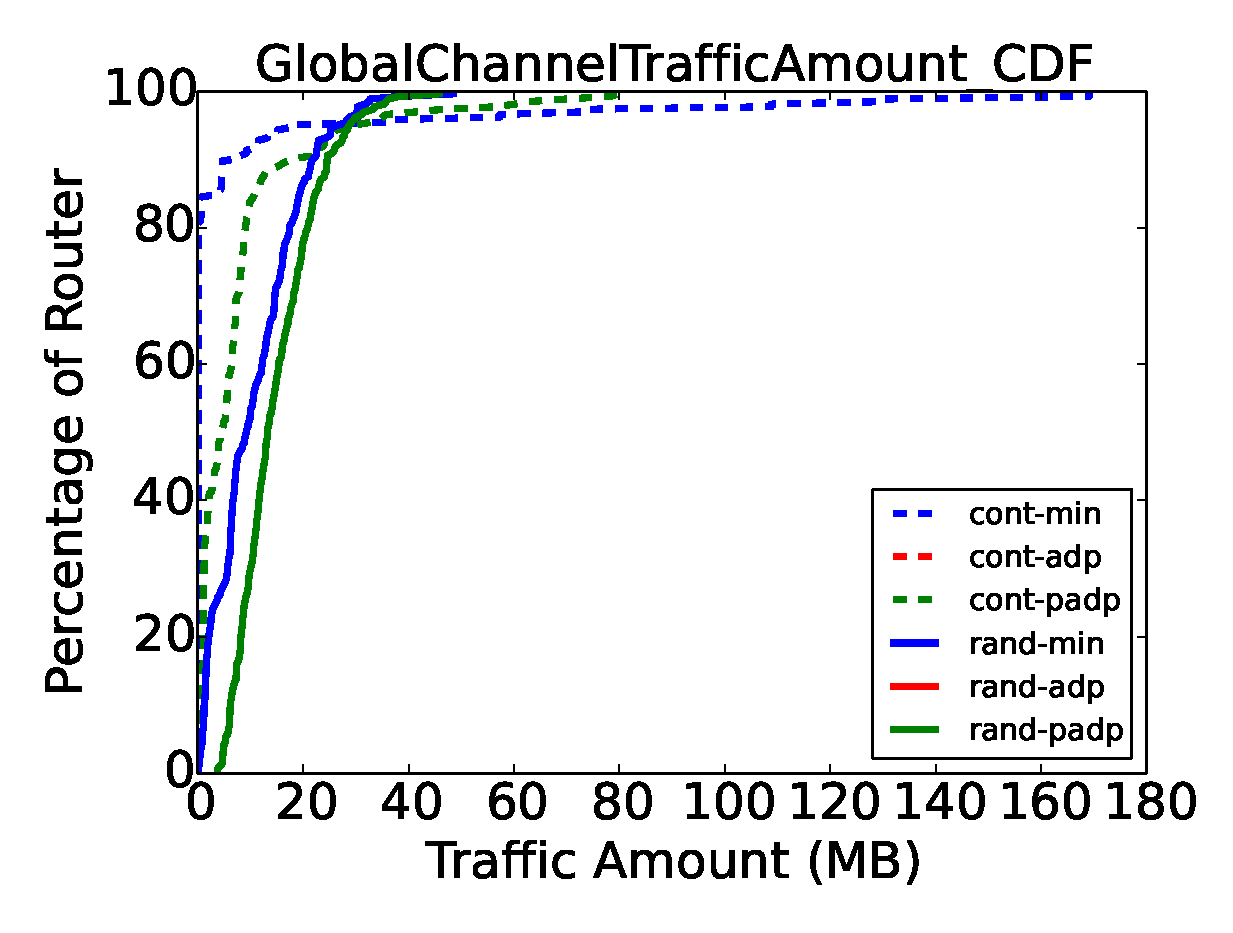
\includegraphics[height=1.8 in]{wkld/gc-traffic}
        \caption{Global Channel Traffic}
        \label{fig:global-channel-traffic}
    \end{subfigure}\hfill
    \hspace{1em}%
    \begin{subfigure}[t]{0.32\textwidth}
        \centering
        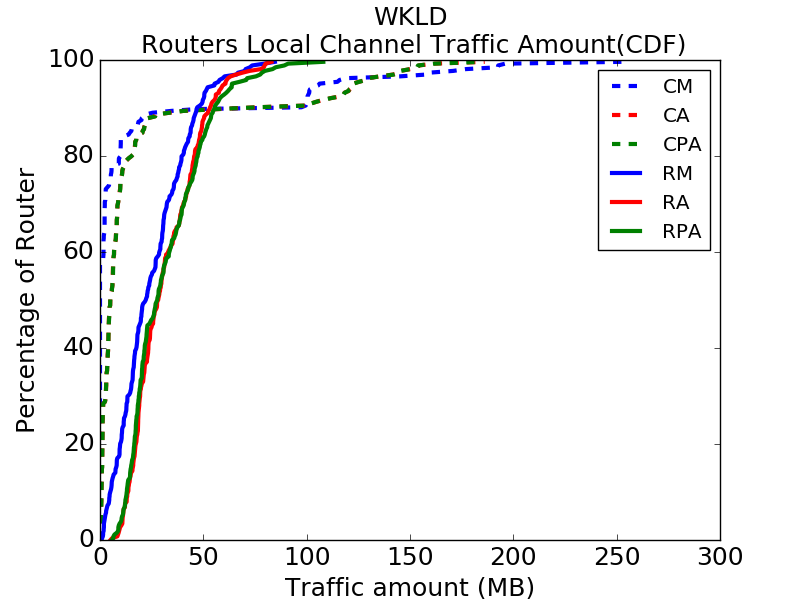
\includegraphics[height=1.8 in]{wkld/lc-traffic}
        \caption{Local Channel Traffic}
        \label{fig:local-channel-traffic}
    \end{subfigure}\hfill
    \hspace{1em}%
    \begin{subfigure}[t]{0.32\textwidth}
        \centering
        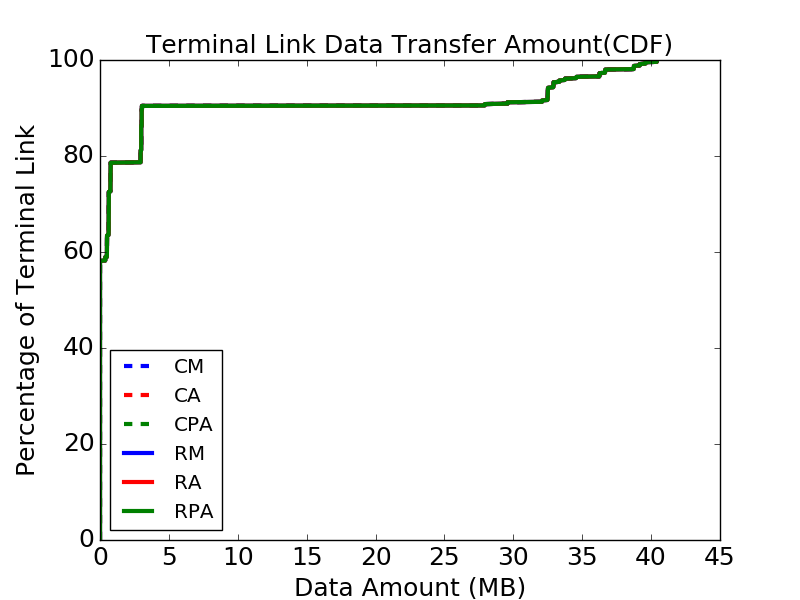
\includegraphics[height=1.8 in]{wkld/tl-traffic}
        \caption{Terminal Link Traffic}
        \label{fig:terminal-link-traffic}
    \end{subfigure}\\

    \centering   
    \begin{subfigure}[t]{0.32\textwidth}
        \centering
        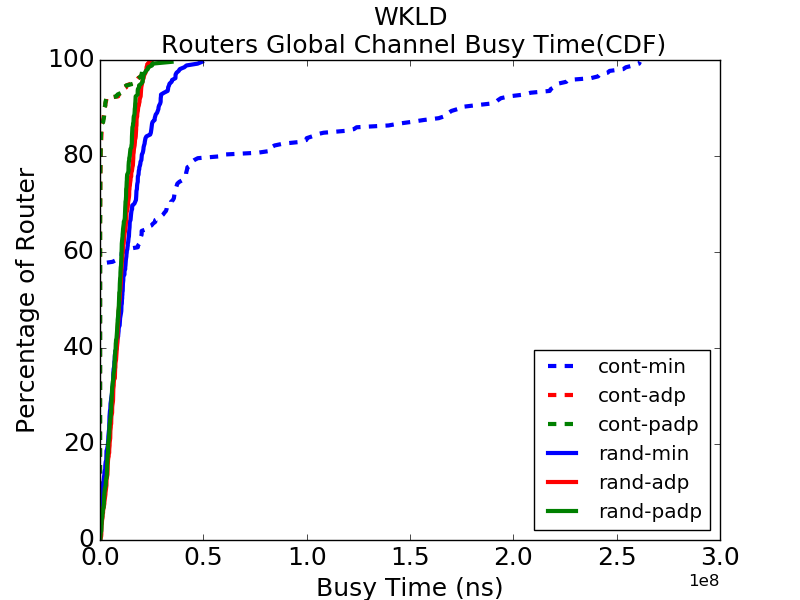
\includegraphics[height=1.8 in]{wkld/gc-stime}
        \caption{Global Channel Saturated Time}
        \label{fig:global-channel-stime}
    \end{subfigure}\hfill
     \hspace{1em}%
    \begin{subfigure}[t]{0.32\textwidth}
        \centering
        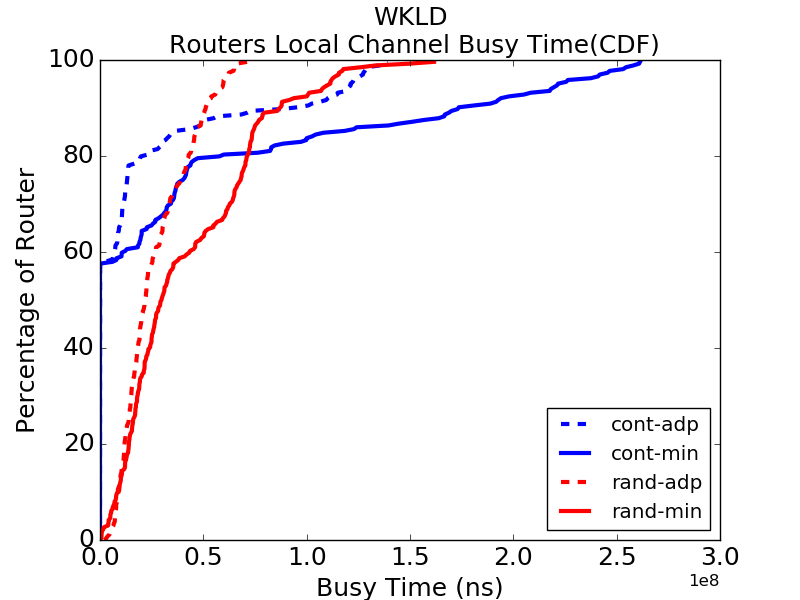
\includegraphics[height=1.8 in]{wkld/lc-stime}
        \caption{Local Channel Saturated Time}
        \label{fig:local-channel-stime}
    \end{subfigure}\hfill
    \hspace{1em}%
    \begin{subfigure}[t]{0.32\textwidth}
        \centering
        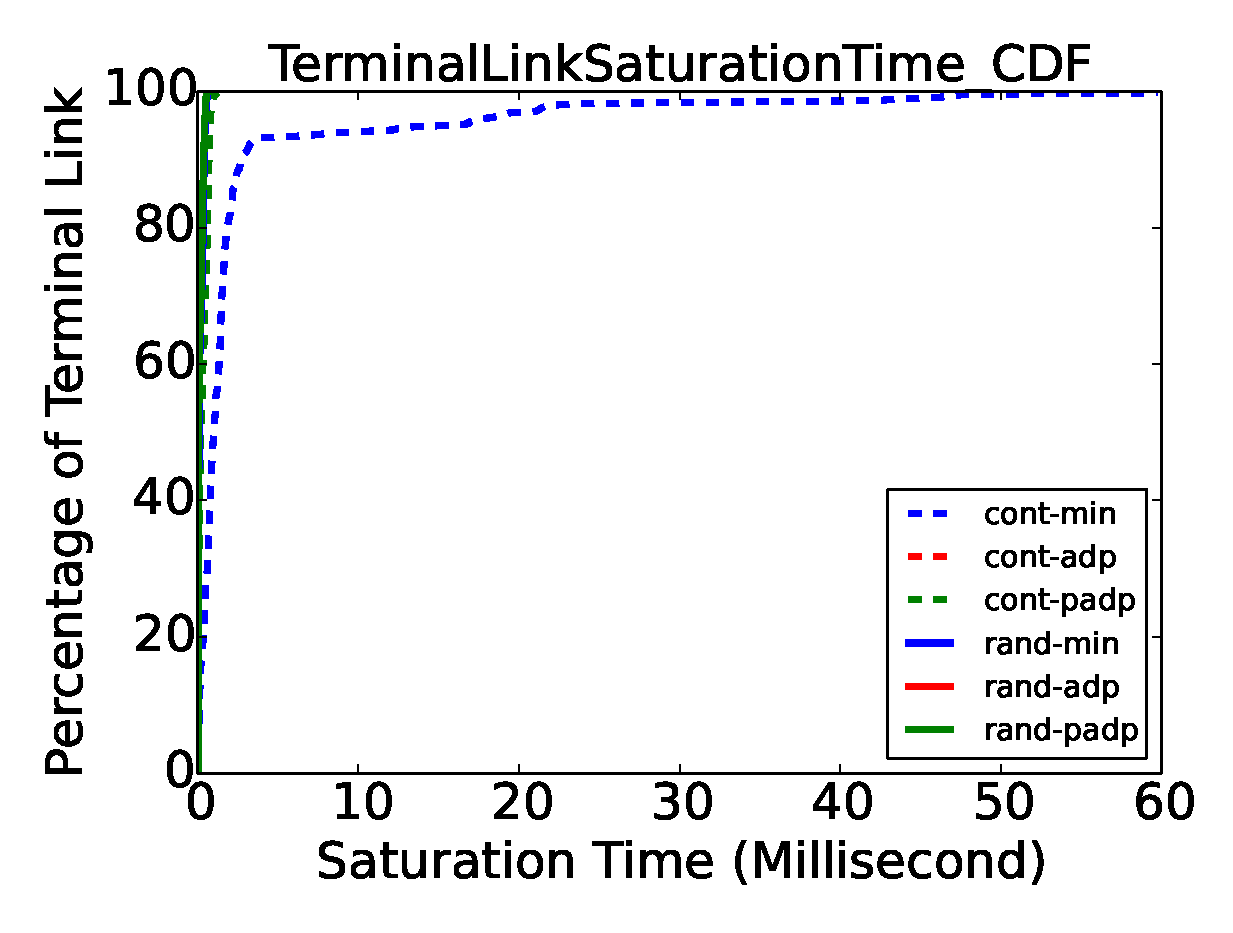
\includegraphics[height=1.8 in]{wkld/tl-stime}
        \caption{Terminal Link Saturated Time}
        \label{fig:terminal-link-stime}
    \end{subfigure}%
   \caption{The aggregate traffic and saturated time of the dragonfly network when Workload \Rmnum{1} running under 6 different placement and routing configurations. ``CA" and ``CPA" performs comparably, the corresponding lines are overlapped. }
   \label{fig:wkld-network-traffic-stime}
\end{figure*}

Figure \ref{fig:wkld-network-traffic-stime} shows the aggregate traffic for terminal links, local channels and global channels as well as the corresponding saturated time when Workload \Rmnum{1} is running on dragonfly network with 6 different placement and routing configurations. When contiguous placement and minimal routing(CM) is in use, all the traffic goes within the contiguously allocated groups, causing congestion along certain shortest paths from source to destination routers. Both the traffic and the corresponding saturated time of global channels are the highest compared with other configurations, shown as the blue dashed line in Figure \ref{fig:global-channel-traffic} and \ref{fig:global-channel-stime}.
When contiguous placement is coupled with (progressive) adaptive routing (CA and CPA), the traffic through congested global channels will be greatly reduced, so does the corresponding saturated time, shown as the red and green dashed line in Figure \ref{fig:global-channel-traffic} and \ref{fig:global-channel-stime}. Since (progressive) adaptive routing are congestion aware, the traffic would be redirected to the intermediate routers in other idle groups when congestion occurs, thus the traffic burden on the contiguously allocated groups will be alleviated. 


Random placement policy performs comparably with three different routing policies.
Shown as the solid lines in Figure \ref{fig:global-channel-traffic}, the traffic through global channels are quite balanced across all the routers, thus no particular global channel will suffer high traffic burden. When the random placements coupled with minimal routing (RM), the packets can avoid unnecessary intermediate forwarding as introduced by (progressive) adaptive routing, thus generating less traffic. That's why the blue solid line is lower than the red and green solid line. Since the random placement can uniformly distribute traffic, there are no sudden surge of saturated time of global channel over the network, shown as solid lines in Figure \ref{fig:global-channel-stime}. 

%local channel traffic and busy time explanation

We observe similar phenomena from the local channel traffic and saturated time, shown in Figure \ref{fig:local-channel-traffic}, \ref{fig:local-channel-stime}). Contiguous placement coupled with minimal routing (CM) results in local congestion, and thus the aggregate traffic through local channels of certain routers is quite high. Even with adaptive or progressive adaptive routing, the local congestion caused by grouping all MPI ranks in the same group(s) in contiguous placement can not be eliminated. Random placement is effective at addressing this type of congestion. 

%terminal link traffic and busy time explanation
Figure \ref{fig:terminal-link-traffic} is for the purpose of symmetry, it shows the traffic per rank (aka traffic through terminal links), which stay the same when different placement and routing configurations are in use. All 6 lines are overlapped in Figure \ref{fig:terminal-link-traffic}. However, due to the traffic changes on global and local channels, the saturated time of terminal links will experience variability when different routing schemes are in use, as shown in Figure \ref{fig:terminal-link-stime}. When contiguous placement coupled with minimal routing(CM), the accumulated congestion on local and global channels cause extremely long saturated time on the terminal link, shown as the blue dashed line in Figure \ref{fig:terminal-link-stime}. This again manifests the severe congestion caused by using contiguous placement and minimal routing. 


\subsection{Individual Application Analysis}
\label{sec: workload-1 app analysis}

\begin{figure*}[t!]
    \centering
    \begin{subfigure}[t]{0.32\textwidth}
        \centering
        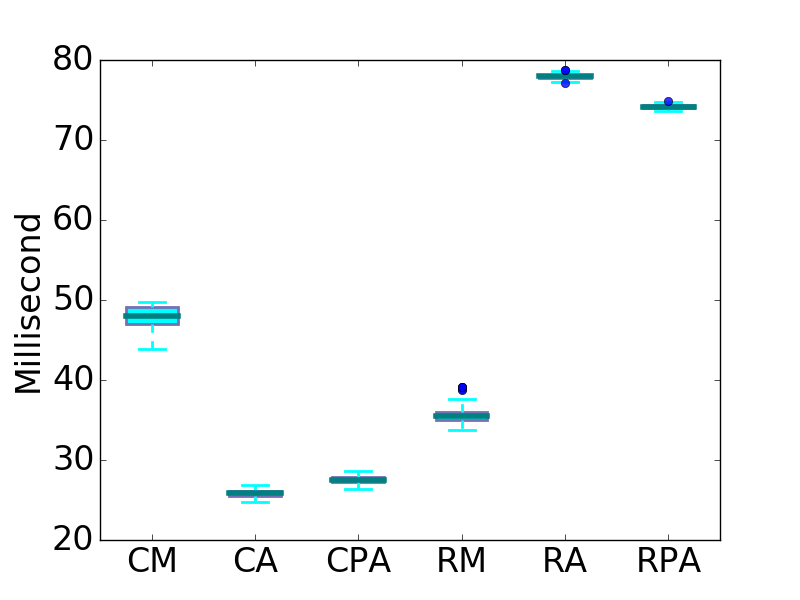
\includegraphics[height=1.5 in]{wkld/amg/commtime}
        \caption{AMG}
        \label{fig:amg-commtime}
    \end{subfigure}%
    \hspace{1em}%
    \begin{subfigure}[t]{0.32\textwidth}
        \centering
        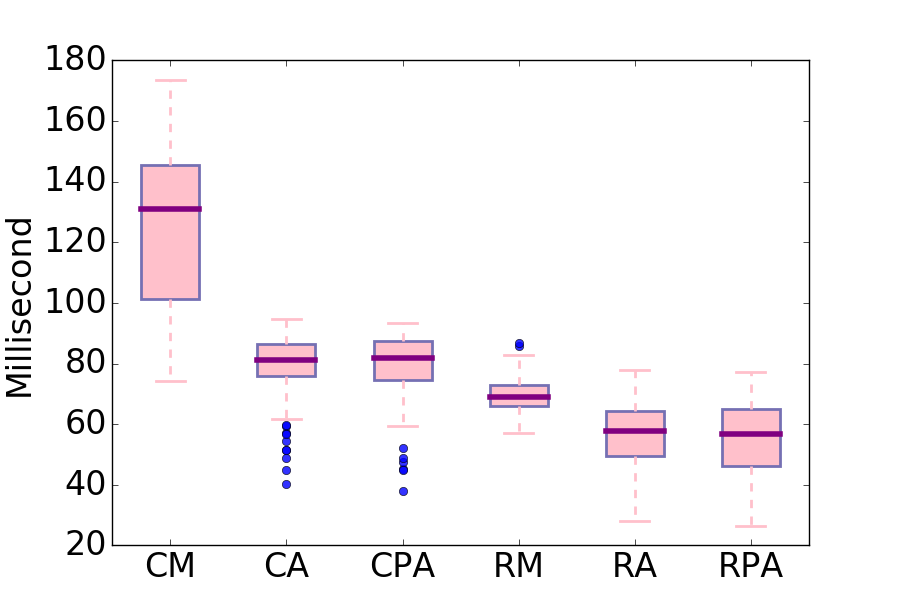
\includegraphics[height=1.5 in]{wkld/mg/commtime}
        \caption{MultiGrid}
        \label{fig:mg-commtime}
    \end{subfigure}%
    \begin{subfigure}[t]{0.32\textwidth}
        \centering
        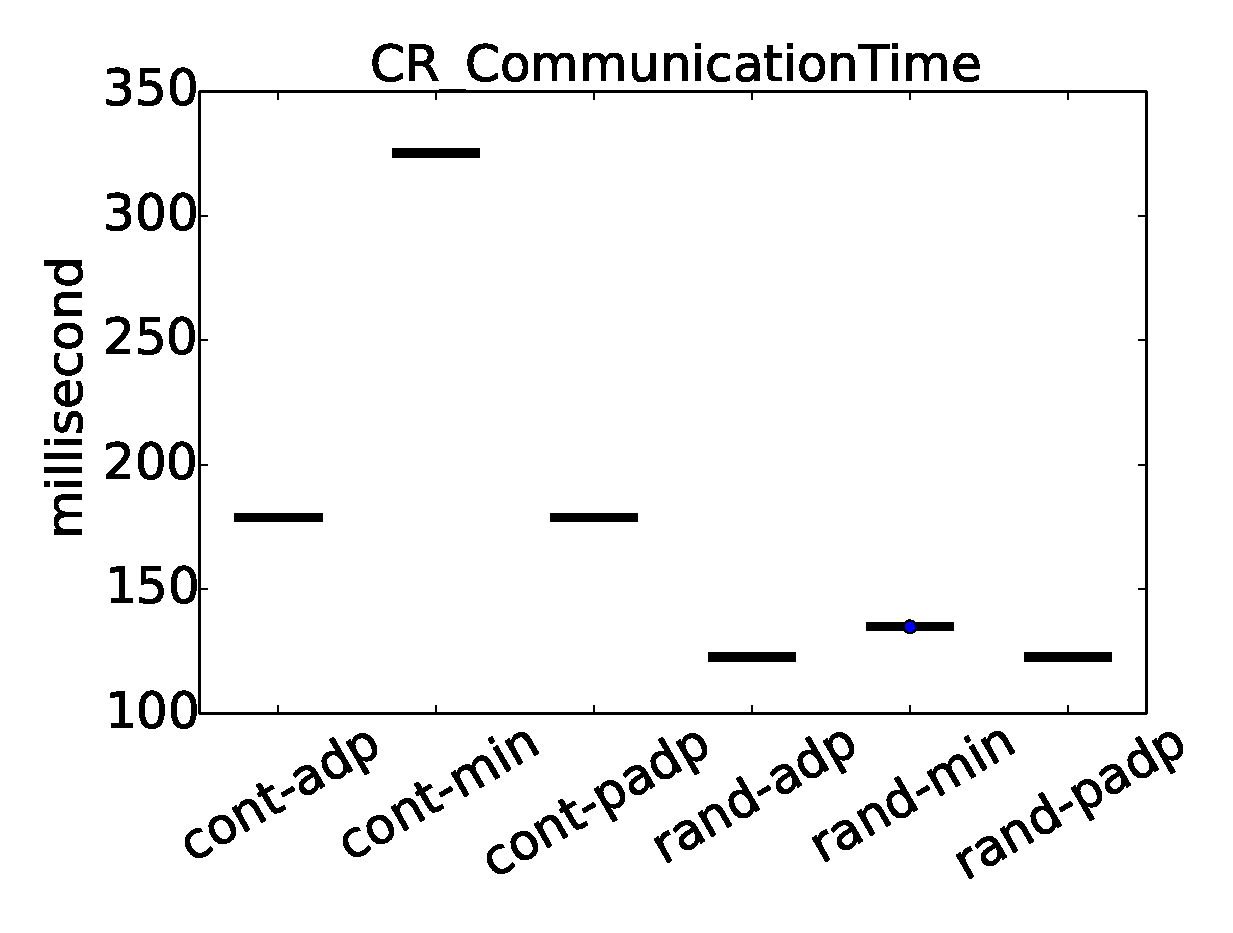
\includegraphics[height=1.5 in]{wkld/cr/commtime}
        \caption{CrystalRouter}
        \label{fig:cr-commtime}
    \end{subfigure}%
   \caption{The communication time of all ranks in each application. Three applications running concurrently on dragonfly network with different placement and routing configurations. Random placement and adaptive routing can improve MG and CR communication, however, AMG's communication time is greatly prolonged.}
   \label{fig:apps-commtime}
\end{figure*}

Figure \ref{fig:apps-commtime} shows the distribution of communication time of three applications in per rank manner, when they running concurrently under 6 different placement and routing configurations listed in Table\ref{tab: placement routing configs}.

As shown in Figure \ref{fig:mg-commtime}, \ref{fig:cr-commtime}, MultiGrid and CrystalRouter suffer the longest communication time when running with contiguous placement and minimal routing (CM). When contiguous placement coupled with adaptive or progressive adaptive routing (CA, CPA), the communication time of both MultiGrid and CrystalRouter are significantly reduced. Random placement further reduces their communication time, and reaches the best performance when coupled with (progressive) adaptive routing (RPA, RA). Both MultiGrid and CrystalRouter show the same trend when they are running under different placement and routing configurations. AMG is quite an exception. The communication time of AMG skyrockets when running under random placement coupled with (progressive) adaptive routing (RPA, RA), shown in Figure \ref{fig:amg-commtime}. The contiguous placement coupled with (progressive) adaptive routing can reach the best performance for AMG. CM is no better than RM, but still much better RPA, RA. 



\begin{figure*}[t]
    \centering
    \begin{subfigure}[t]{0.32\textwidth}
        \centering
        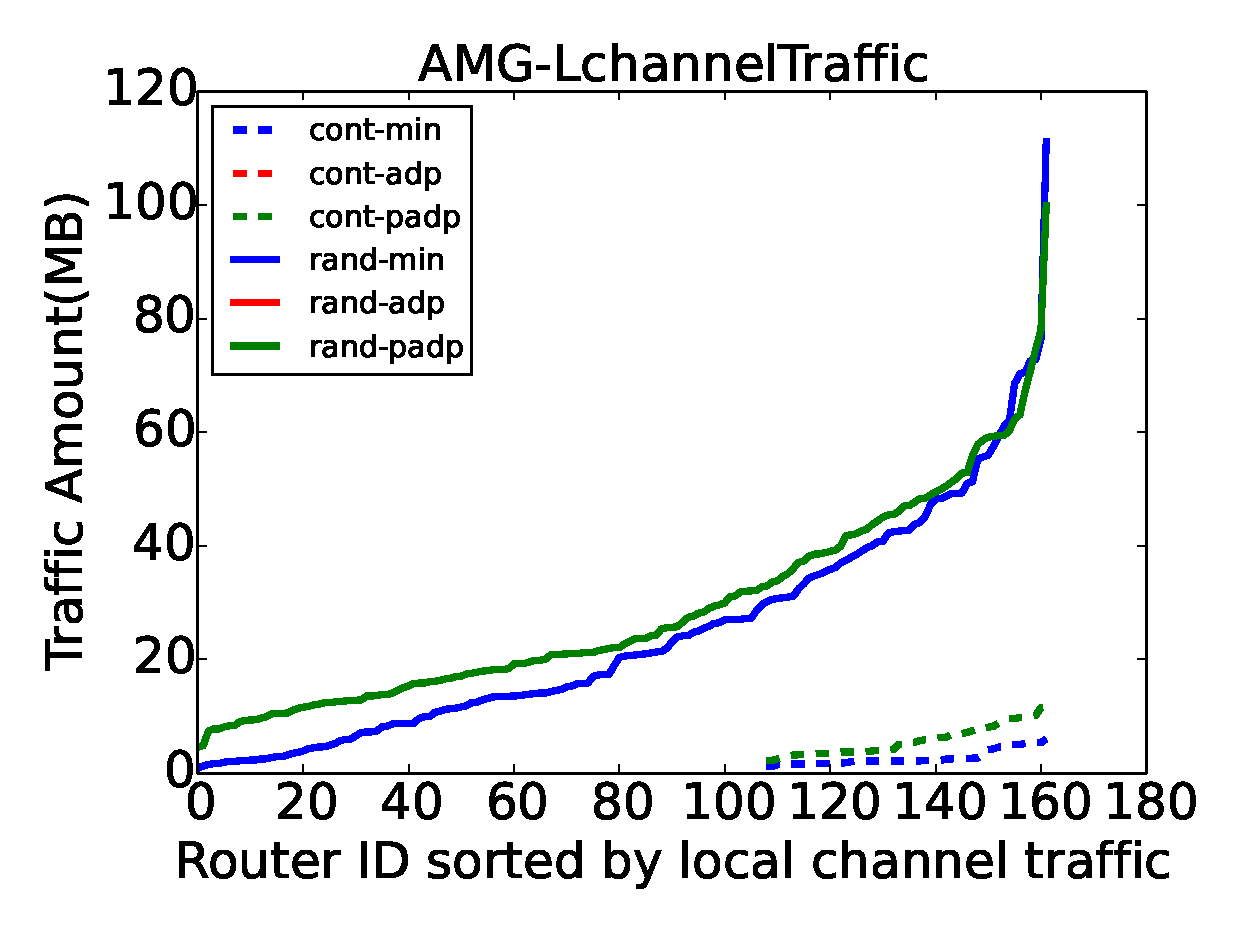
\includegraphics[height=1.8 in]{wkld/amg/lc-traffic}
        \caption{AMG Local Channel Traffic}
        \label{fig:amg-lc-traffic}
    \end{subfigure}\hfill
    \hspace{1em}%
    \begin{subfigure}[t]{0.32\textwidth}
        \centering
        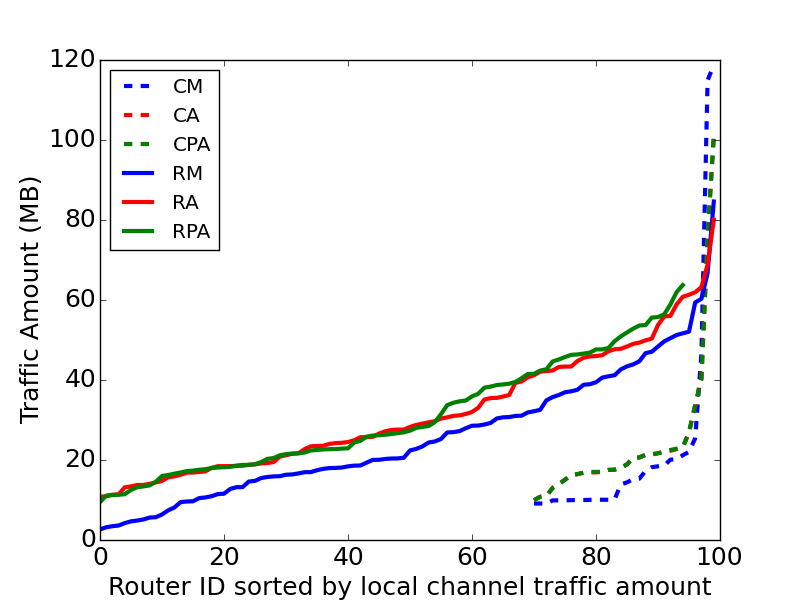
\includegraphics[height=1.8 in]{wkld/mg/lc-traffic}
        \caption{MG Local Channel Traffic}
        \label{fig:mg-lc-traffic}
    \end{subfigure}\hfill
    \begin{subfigure}[t]{0.32\textwidth}
        \centering
        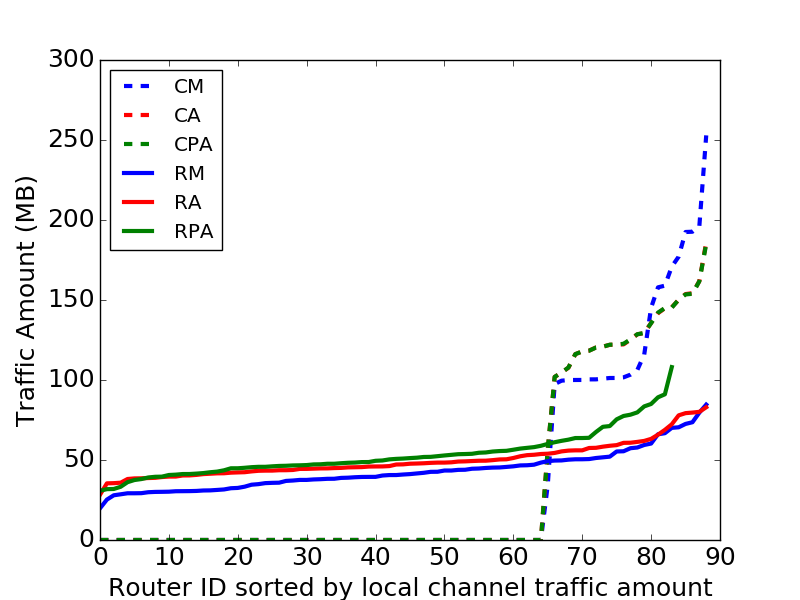
\includegraphics[height=1.8 in]{wkld/cr/lc-traffic}
        \caption{CR Local Channel Traffic}
        \label{fig:cr-lc-traffic}
    \end{subfigure}\\
    \centering
    \begin{subfigure}[t]{0.32\textwidth}
        \centering
        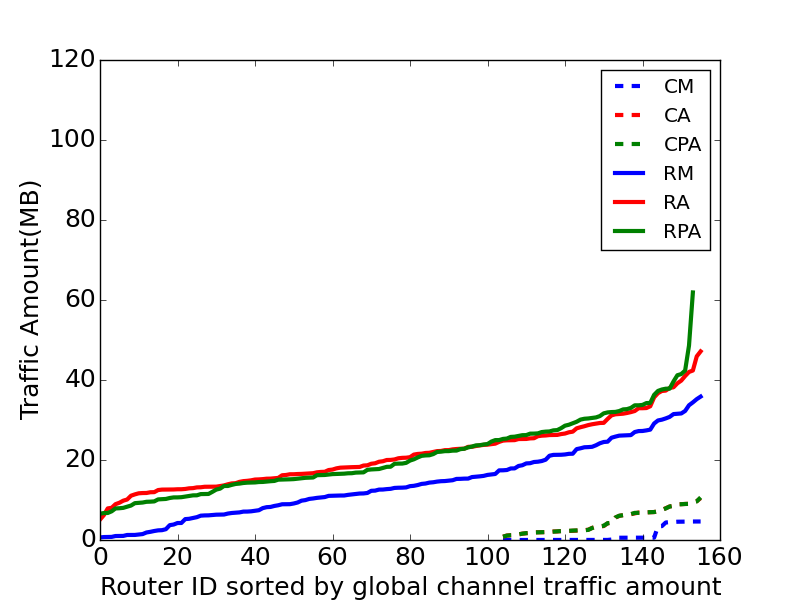
\includegraphics[height=1.8 in]{wkld/amg/gc-traffic}
        \caption{AMG Global Channel Traffic}
        \label{fig:amg-gc-traffic}
    \end{subfigure}\hfill
    \hspace{1em}%
    \begin{subfigure}[t]{0.32\textwidth}
        \centering
        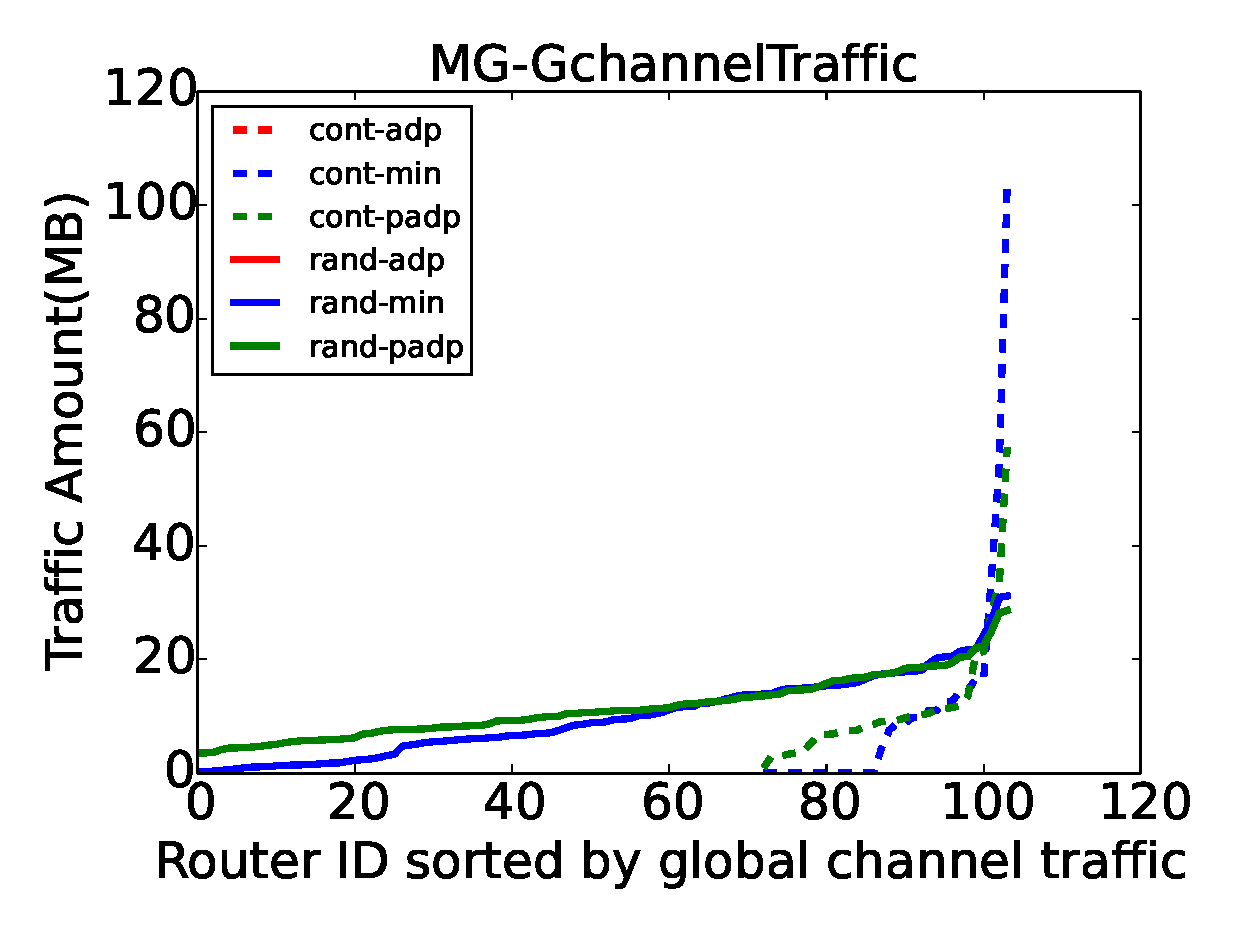
\includegraphics[height=1.8 in]{wkld/mg/gc-traffic}
        \caption{MG Global Channel Traffic}
        \label{fig:mg-gc-traffic}
    \end{subfigure}\hfill
    \begin{subfigure}[t]{0.32\textwidth}
        \centering
        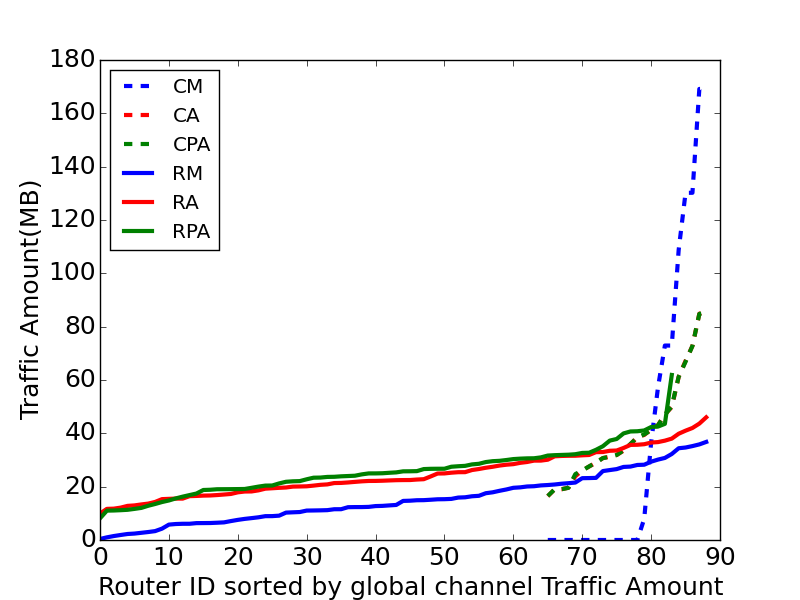
\includegraphics[height=1.8 in]{wkld/cr/gc-traffic}
        \caption{CR Global Channel Traffic}
        \label{fig:cr-gc-traffic}
    \end{subfigure}%
   \caption{The aggregate traffic go through the local and global channels of routers serving specific application. ``CA" and ``CPA" perform comparably, the corresponding lines are overlapped. More routers are involved in serving each application when random placement is in use, compared with contiguous placement.}
   \label{fig:3app-lc-gc-traffic}
\end{figure*}


% Show the evidence from network level, explain why AMG is different. 
We look into network level to identify the culprit behind AMG's abnormal behavior with random placement and adaptive routing. By identifying the compute nodes each MPI rank resides on and routers that serving each application, we can see that the traffic go through the routers serving AMG skyrockets when random placement and adaptive routing is in use, shown in Figure \ref{fig:amg-lc-traffic} and \ref{fig:amg-gc-traffic}. Adaptive routing will redirect the traffic of other applications to go through the routers belonging to AMG, and increase the traffic burden on those routers, thus slow down the communication of AMG.

No router will be shared between applications under contiguous placement. A number of successive groups will be allocated to the same application under contiguous placement policy. When contiguous placement coupled with minimal routing, application will be free of interference from its concurrently running peers. However, application communication traffic will be confined within their allocated groups, thus congestion is very likely to happen depending on application communication intensity. As the lest communication-intensive application in Workload \Rmnum{1}, AMG can benefit from contiguous placement. Under contiguous placement, the traffic go through the local and global channels of the routers belonging to AMG is significantly lower than with random placement, shown in Figure \ref{fig:amg-lc-traffic}, \ref{fig:amg-gc-traffic}. 

MultiGrid and CrystalRouter are more communication-intensive compared with AMG. They will suffer congestion on both local and global channels when contiguous placement is in use, shown as the dashed line in Figure \ref{fig:mg-lc-traffic}, \ref{fig:mg-gc-traffic} and Figure \ref{fig:cr-lc-traffic}, \ref{fig:cr-gc-traffic}. On the other hand, the random placement can uniformly distribute their traffic all over the network, alleviate the possible congestion, shown as the solid lines in Figure \ref{fig:mg-lc-traffic}, \ref{fig:mg-gc-traffic} and Figure \ref{fig:cr-lc-traffic}, \ref{fig:cr-gc-traffic}.


\subsection{Key Observations}
In summary, based on the results presented in section \ref{sec: workload-1 network analysis} and \ref{sec: workload-1 app analysis}, we have made the following observations.


\emph{Network performance will be significantly improved when random placement and adaptive routing are in use.} Random placement can uniformly distribute MPI ranks of application over the network, and adaptive routing can redirect the traffic from congested routers to other less busy routers. Therefore, the network could reach the status of load-balanced and hot-spots free. 

\emph{The performance of less communication-intensive jobs in workload will suffer degradation when network random placement and adaptive routing are in use.} AMG in Workload \Rmnum{1} are ``bullied" by their concurrently running communication-intensive peers, MultiGrid and CrystalRouter. AMG shares routers and groups with MultiGrid and CrystalRouter when random placement is in use. The traffic from MultiGrid and CrystalRouter will be redirected to the routers that serving AMG, slowing down AMG's communication. \footnote{We have tried three different congestion sensing schemes that used in adaptive routing\cite{won-prog-adaptive}, although there are some variations between the results, none of the congestion sensing scheme can prevent the ``bully" from happening.}

\emph{Consistent performance of each application can be guaranteed when contiguous placement and minimal routing are in use.} The router and group sharing between jobs are prohibited in contiguous placement policy. The traffic won't be redirected from congested routers to less busy ones when minimal routing is in use. Thus the interference between concurrently running jobs will be eliminated and the ``bully" behavior will be terminated. 
%However, contiguous placement and minimal routing usually results in local congestion and unbalanced network utilization.


\section{Study of Parallel Workload \Rmnum{2 }}
%\section{``Bully" become ``Bullee"}
\label{sec:workload-2}

In this section, we will verify the observations made in the previous section when Workload \Rmnum{1} is running on the dragonfly network under different placement and routing configurations. We conduct the same sets of experiments with Workload \Rmnum{2}, which consists of sAMG, MultiGrid and CrystalRouter. By replacing AMG with sAMG, we turn the ``bully" into ``bullee".

\subsection{Network Performance Analysis}
\label{sec: workload-2 network analysis}

\begin{table}[ht]
\begin{center}
\caption{Average time spent on communication by all MPI ranks when Workload II is running on dragonfly network under 6 different placement and routing configurations.} 
\label{tab:syn-wkld-commtime}
%\centering % Centers the table on the page, comment out to left-justify
\begin{tabular}{l c c c c c c }
\toprule % Top horizontal line
\toprule
&\multicolumn{6}{c}{Placement and Routing Configuration} \\ % Amalgamating several columns into one cell is done using the \multicolumn command as seen on this line
\cmidrule(l){2-7}
	      & CM & CA & CPA & RM & RA & RPA \\ % Column names row
\midrule % In-table horizontal line
Time(ms)  & 3360 & 2204 & 2335 & 1791 & 2367 & 1965 \\ % Content row 1

\midrule % In-table horizontal line
\bottomrule % Bottom horizontal line
\end{tabular}
\end{center}
\end{table}


The average communication time spent by all MPI ranks when Workload \Rmnum{2} is running under different placement and routing configurations shown in Table \ref{tab:syn-wkld-commtime}. The contiguous placement coupled with minimal routing results in highest communication time. The random placement coupled with minimal routing is the most efficient. Progressive adaptive routing is better than adaptive routing when random placement is in use. And they have comparable results when coupled contiguous placement. The performance of Workload \Rmnum{2} under different configurations keep the similar pattern as it of Workload \Rmnum{1}. 


Figure \ref{fig:synwkld-network-traffic-stime} shows the aggregate traffic for terminal links, local channels and global channels, and the corresponding saturated time when Workload \Rmnum{2} is running with 6 different configurations. Contiguous placement coupled with minimal routing(CM) results in most traffic go through certain local and global channel, thus the longest saturated time for terminal link, local and global channel. When contiguous placement is coupled with (progressive) adaptive routing (CA, CPA), the local congestion could be mitigated. The random placement coupled with any routing policy(RM, RA, RPA) performs comparably. They are better than contiguous placement and minimal routing(CM), but only little improvement against contiguous and (progressive) adaptive (CA, CPA).



\begin{figure*}[t]
    \centering
    \begin{subfigure}[t]{0.32\textwidth}
        \centering
        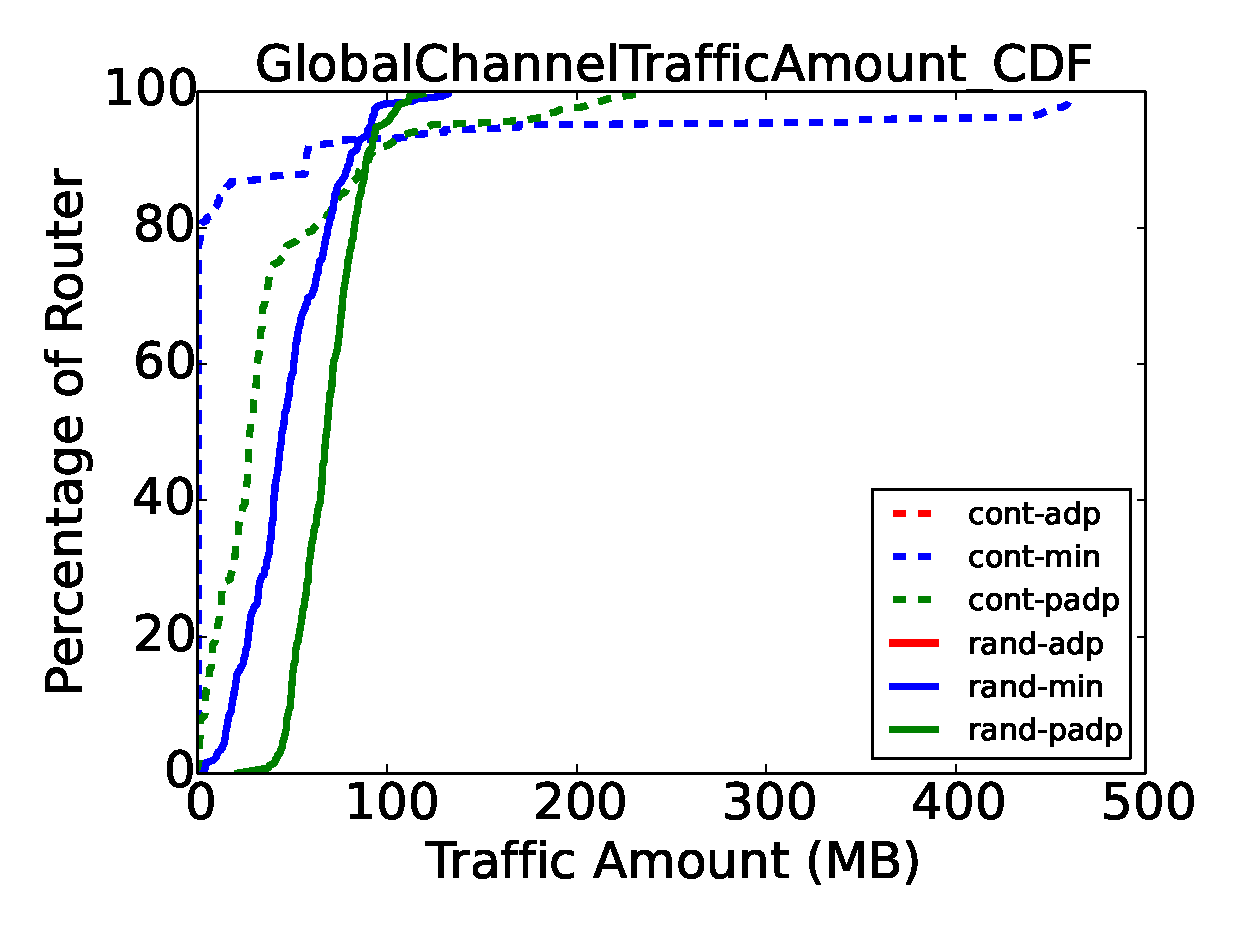
\includegraphics[height=1.8 in]{syn-wkld/gc-traffic}
        \caption{Global Channel Traffic}
        \label{fig:synwkld-global-channel-traffic}
    \end{subfigure}\hfill
    \hspace{1em}%
    \begin{subfigure}[t]{0.32\textwidth}
        \centering
        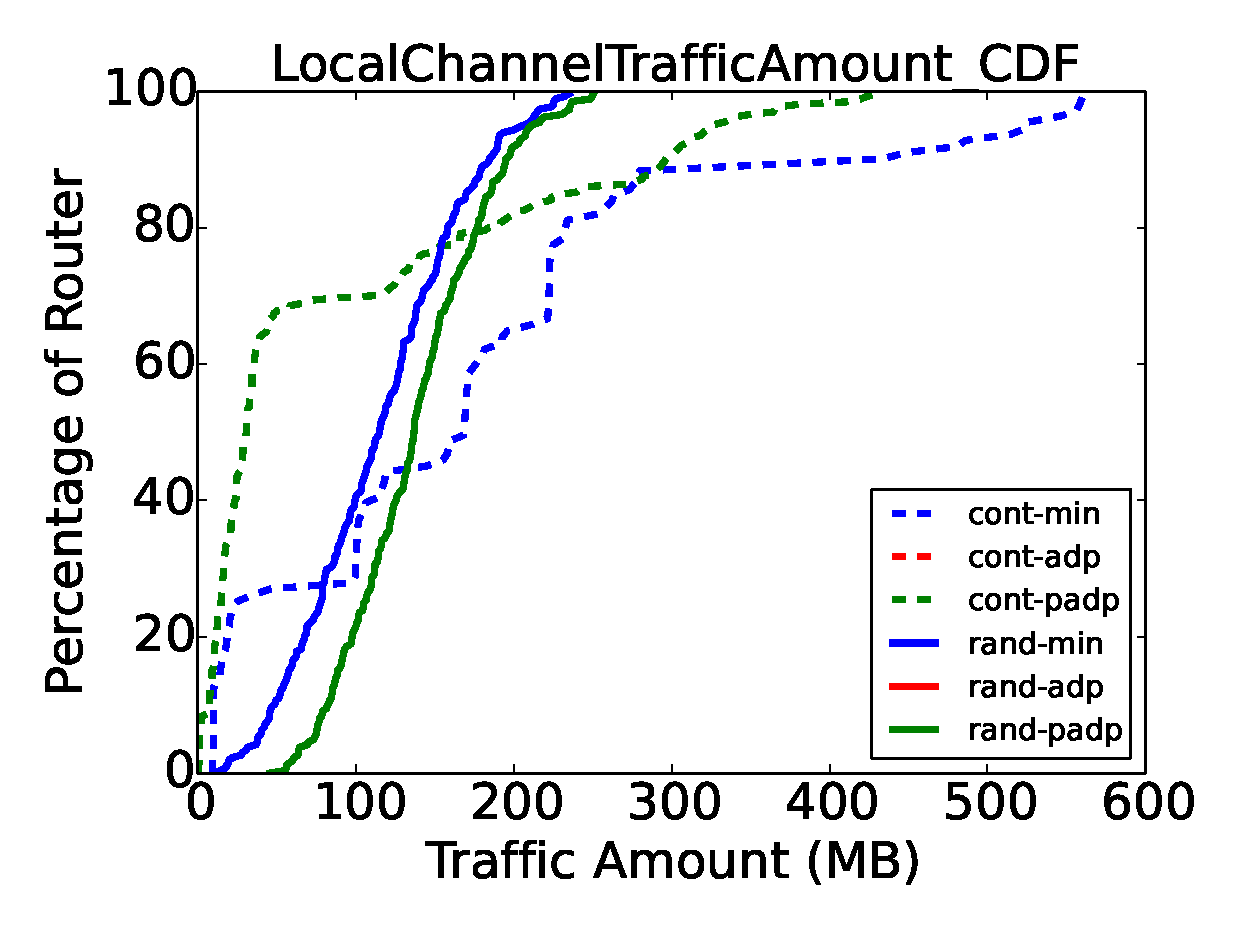
\includegraphics[height=1.8 in]{syn-wkld/lc-traffic}
        \caption{Local Channel Traffic}
        \label{fig:synwkld-local-channel-traffic}
    \end{subfigure}\hfill
    \hspace{1em}%
    \begin{subfigure}[t]{0.32\textwidth}
        \centering
        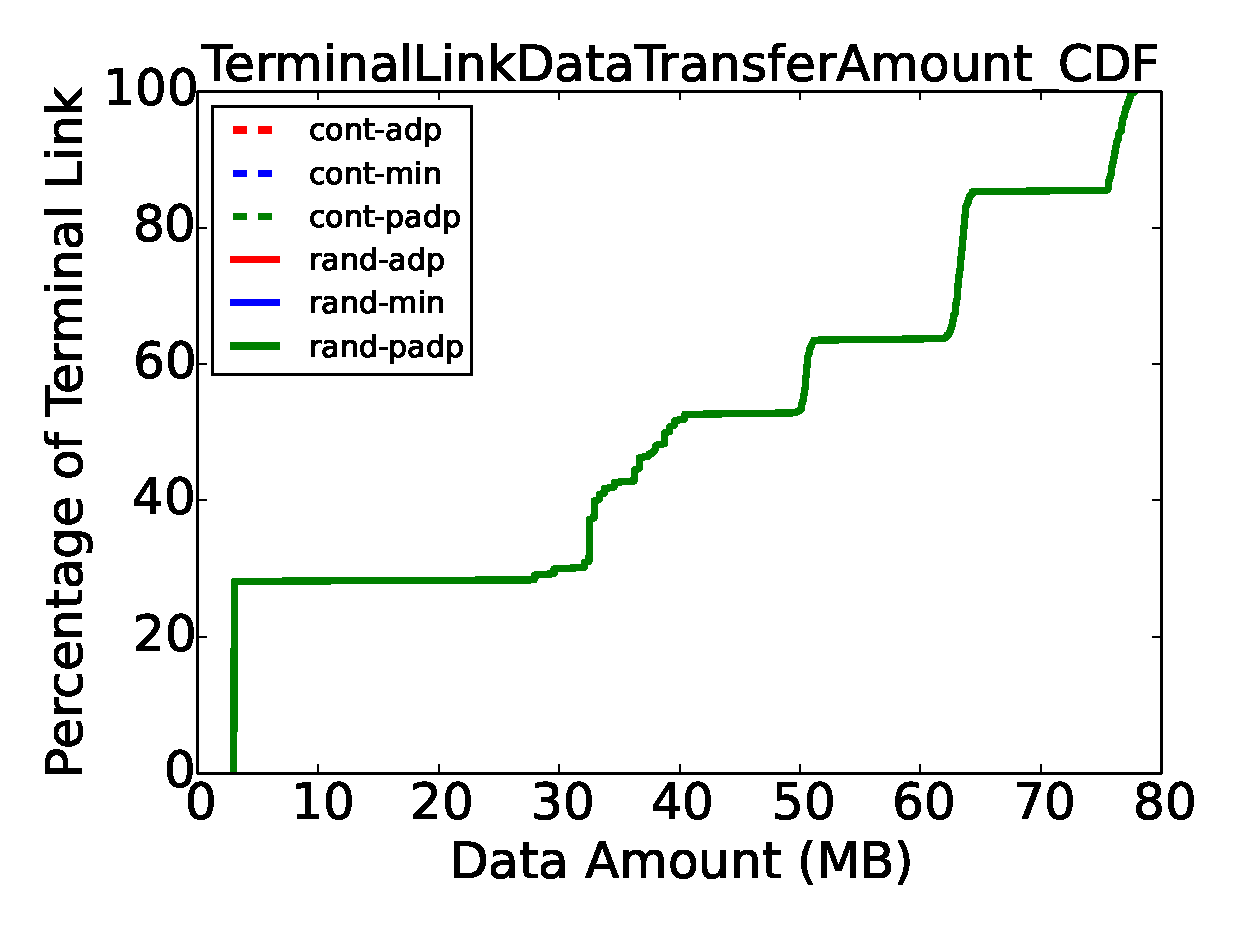
\includegraphics[height=1.8 in]{syn-wkld/tl-traffic}
        \caption{Terminal Link Traffic}
        \label{fig:synwkld-terminal-link-traffic}
    \end{subfigure}\\

    \begin{subfigure}[t]{0.32\textwidth}
        \centering
        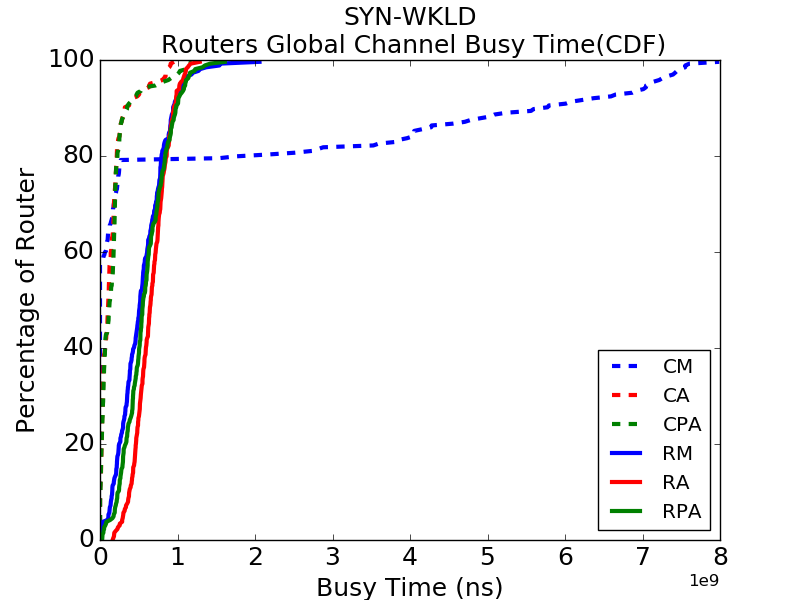
\includegraphics[height=1.8 in]{syn-wkld/gc-btime}
        \caption{Global Channel Saturated Time}
        \label{fig:synwkld-global-channel-stime}
    \end{subfigure}\hfill
     \hspace{1em}%
    \begin{subfigure}[t]{0.32\textwidth}
        \centering
        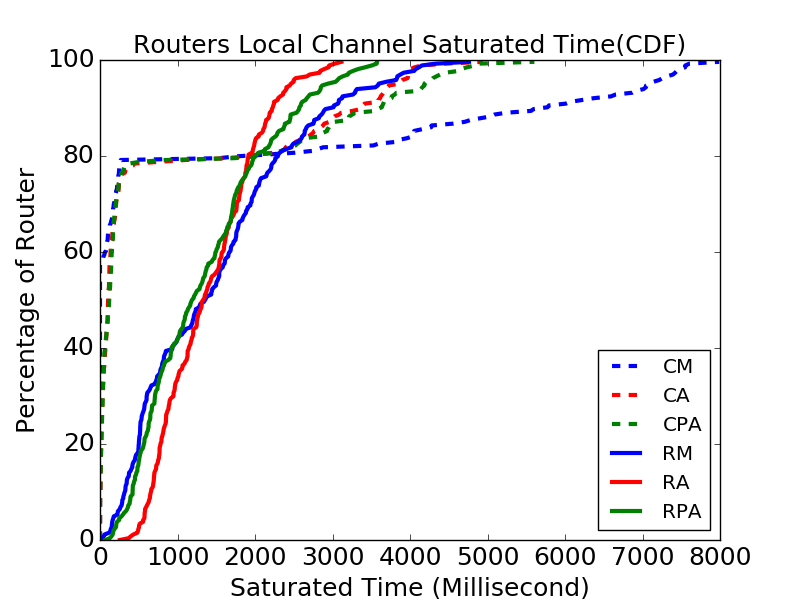
\includegraphics[height=1.8 in]{syn-wkld/lc-btime}
        \caption{Local Channel Saturated Time}
        \label{fig:synwkld-local-channel-stime}
    \end{subfigure}\hfill
    \hspace{1em}%
    \begin{subfigure}[t]{0.32\textwidth}
        \centering
        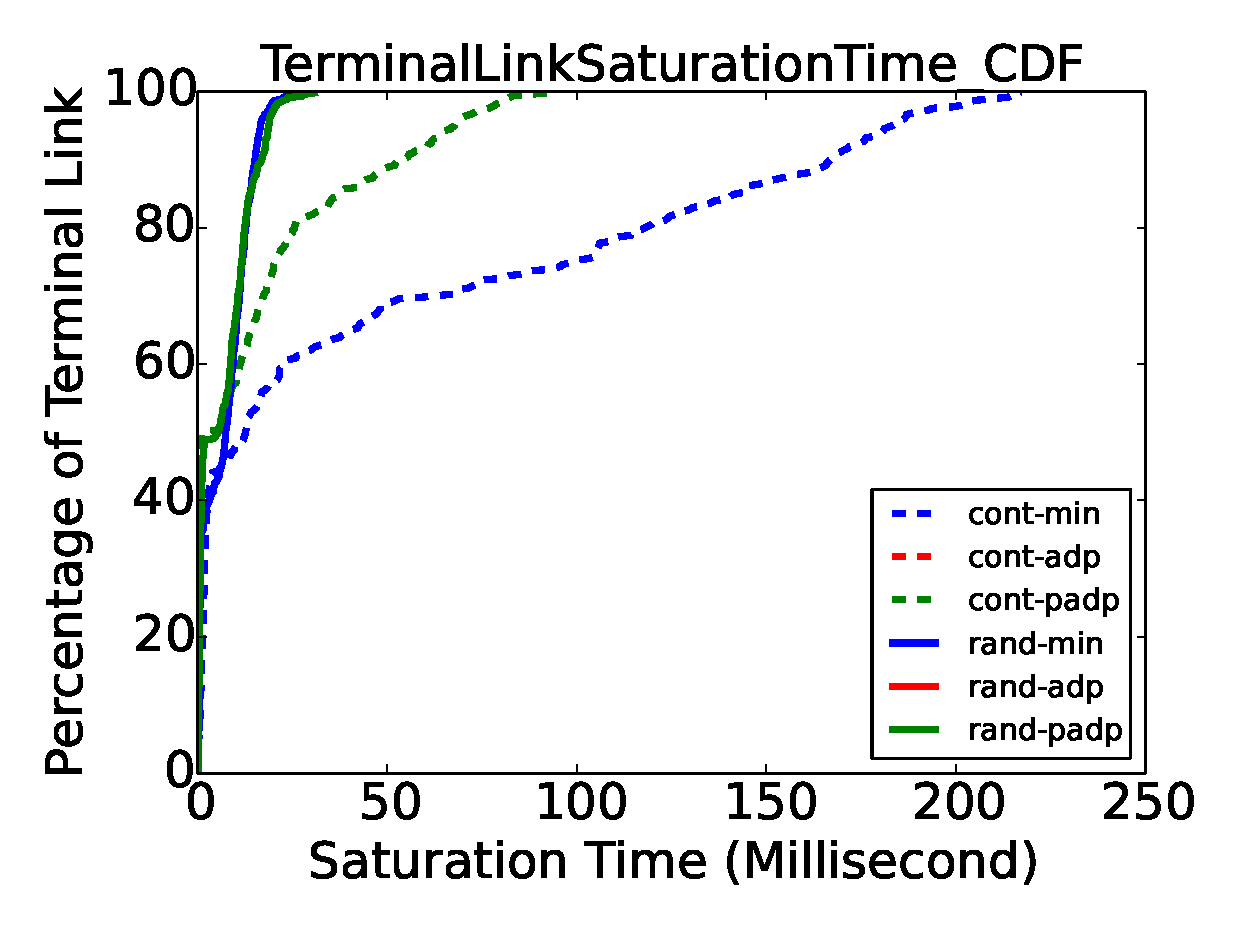
\includegraphics[height=1.8 in]{syn-wkld/tl-btime}
        \caption{Terminal Link Saturated Time}
        \label{fig:synwkld-terminal-link-stime}
    \end{subfigure}%
   \caption{Traffic and Saturated Time of different level of links in the dragonfly network when Workload \Rmnum{2} is running under 6 different placement and routing configurations.}
   \label{fig:synwkld-network-traffic-stime}
\end{figure*}

\subsection{Individual Application Analysis}
\label{sec: workload-2 app analysis}

The communication time of each application shown in Figure \ref{fig:syn-apps-commtime}. The ``bully" in Workload \Rmnum{1} becomes the ``bullyee" in Workload \Rmnum{2}. MultiGrid and CrystalRouter are the less communication-intensive applications in Workload \Rmnum{2}.  When random placement coupled with (progressive) adaptive routing is in use, MultiGrid and CrystalRouter suffer prolonged communication time, shown in Figure \ref{fig:syn-mg-commtime}, \ref{fig:syn-cr-commtime}. Whereas, sAMG benefits from random placement and (progressive) adaptive routing, shown in Figure \ref{fig:syn-samg-commtime}. Contiguous placement coupled with minimal routing prevents applications from sharing network resource, guaranteeing the performance of less communication intensive applications like MultiGrid and CrystalRouter and causing severe performance degradation to sAMG.

\begin{figure*}[t!]
    \centering
    \begin{subfigure}[t]{0.32\textwidth}
        \centering
        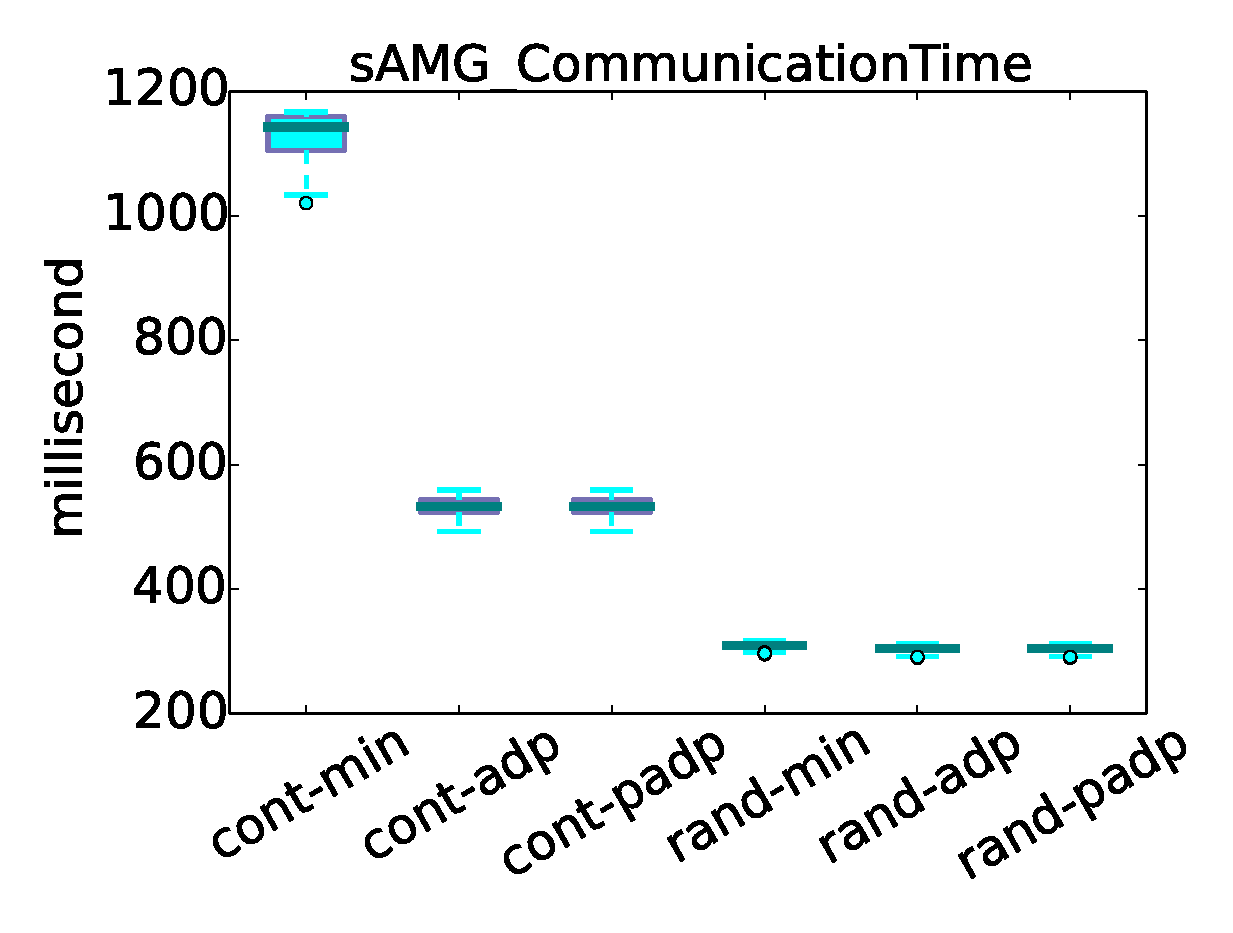
\includegraphics[height=1.5 in]{syn-wkld/amg10/commtime}
        \caption{sAMG}
        \label{fig:syn-samg-commtime}
    \end{subfigure}%
    \hspace{1em}%
    \begin{subfigure}[t]{0.32\textwidth}
        \centering
        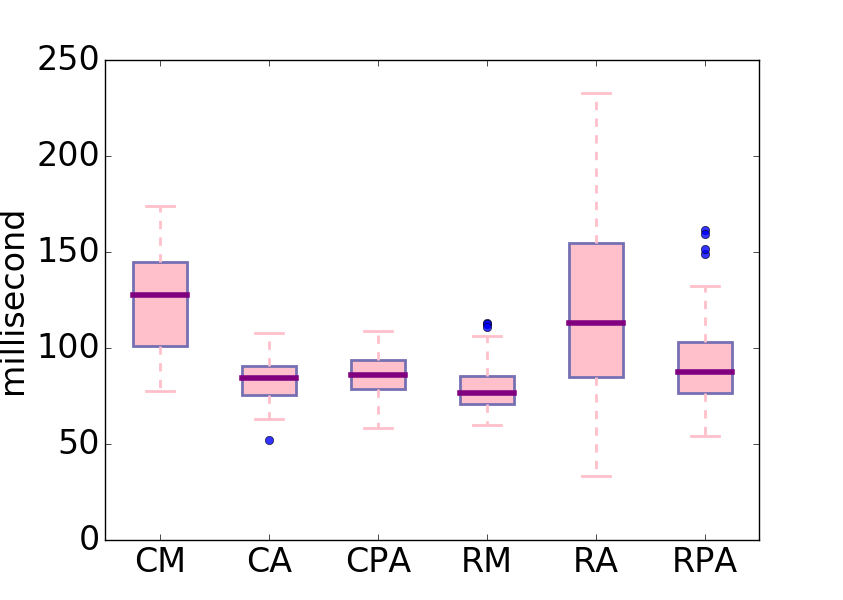
\includegraphics[height=1.5 in]{syn-wkld/mg/commtime}
        \caption{MultiGrid}
        \label{fig:syn-mg-commtime}
    \end{subfigure}%
    \begin{subfigure}[t]{0.32\textwidth}
        \centering
        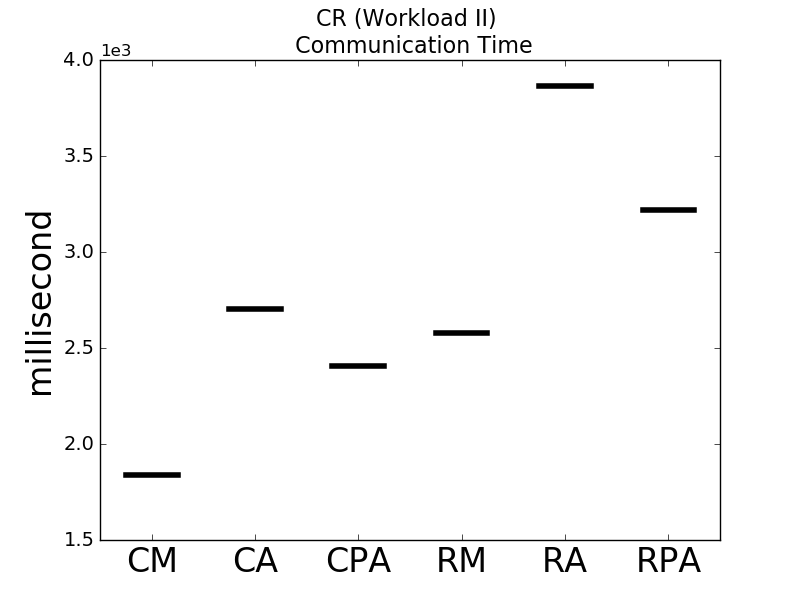
\includegraphics[height=1.5 in]{syn-wkld/cr/commtime}
        \caption{CrystalRouter}
        \label{fig:syn-cr-commtime}
    \end{subfigure}%
   \caption{The communication time of all ranks in each application. Three applications running concurrently on dragonfly network with different placement and routing configurations. The ``bully", sAMG, benefits from random placement and adaptive routing, while the ``bullee", MultiGrid and CrystalRouter, suffer performance degradation.}
   \label{fig:syn-apps-commtime}
\end{figure*}

% explain the network status of sAMG, MG and CR
We look into the network level to scrutinize the traffic through the routers serving each application. Figure \ref{fig:syn-samg-lc-traffic}, \ref{fig:syn-samg-gc-traffic} shows the traffic go through the local and global channels of the routers serving sAMG. The traffic skyrockets in both local and global channels when contiguous placement coupled with minimal routing (CM) is in use. The congestion will be alleviated in both local and global channels when contiguous placement coupled with (progressive) adaptive routing (CA, CPA) are in use. Random placement can further reduce the traffic burden on local and global channels by uniformly distributing sAMG traffic over the network. 

The traffic go through the local and global channels of the routers serving MultiGrid and CrystalRouter are shown in Figure \ref{fig:syn-mg-lc-traffic}, \ref{fig:syn-mg-gc-traffic} and Figure \ref{fig:syn-cr-lc-traffic}, \ref{fig:syn-cr-gc-traffic}. There are more traffic going through when random placement is in use, compared with contiguous placement. The extra traffic coming from the ``bully" sAMG cause performance degradation to MultiGrid and CrystalRouter. 


\begin{figure*}[t]
    \centering
    \begin{subfigure}[t]{0.32\textwidth}
        \centering
        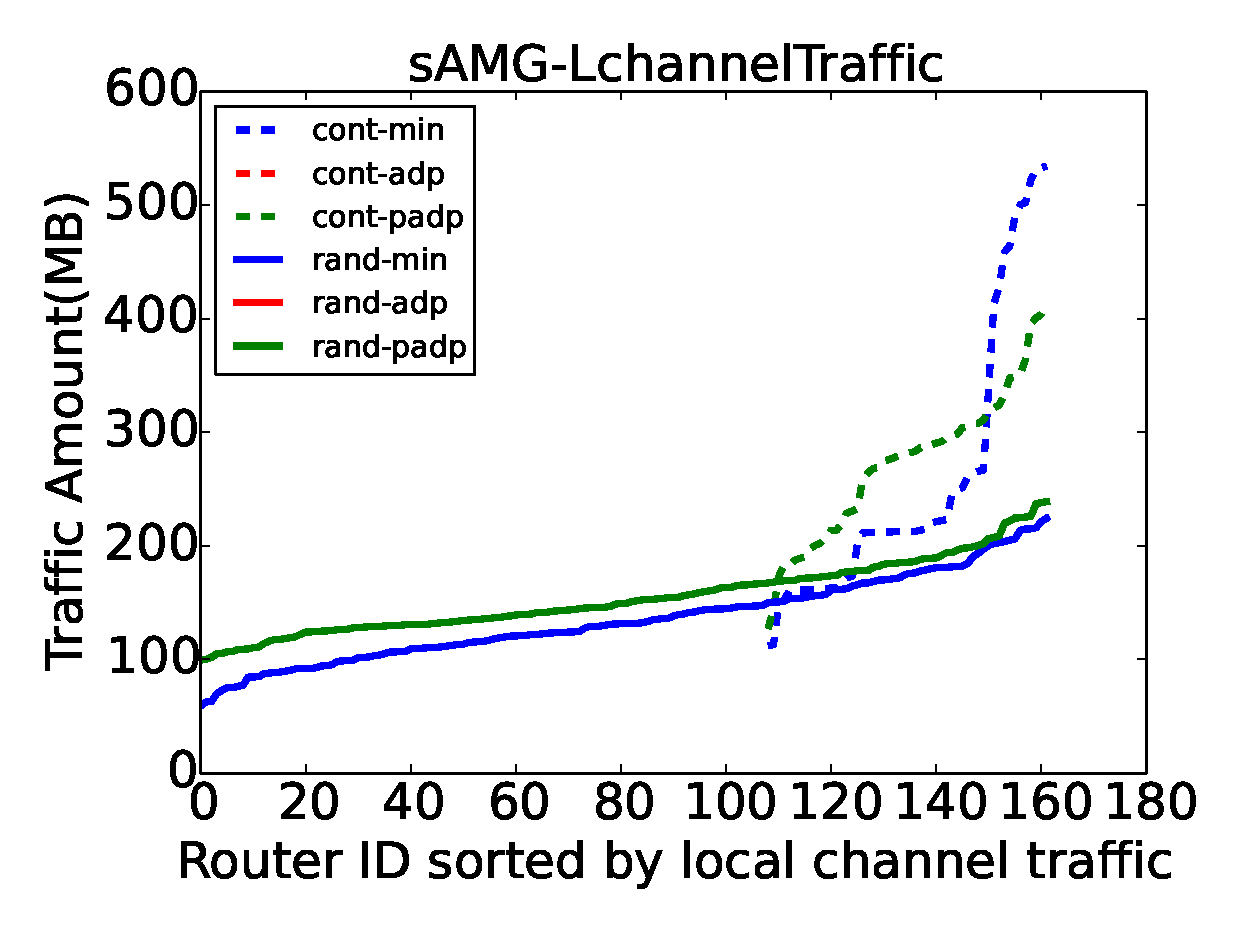
\includegraphics[height=1.5 in]{syn-wkld/amg10/lc-traffic}
        \caption{sAMG Local Channel Traffic}
        \label{fig:syn-samg-lc-traffic}
    \end{subfigure}\hfill
    \hspace{1em}%
    \begin{subfigure}[t]{0.32\textwidth}
        \centering
        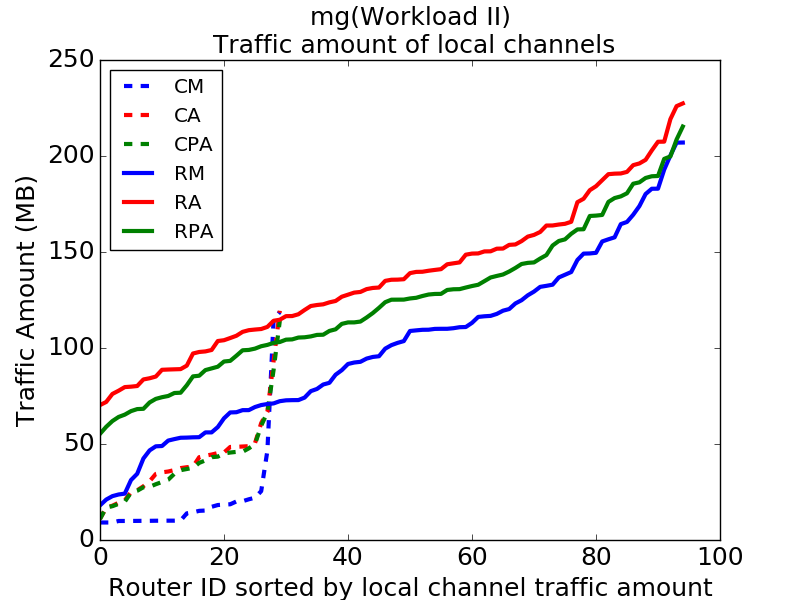
\includegraphics[height=1.5 in]{syn-wkld/mg/lc-traffic}
        \caption{MG Local Channel Traffic}
        \label{fig:syn-mg-lc-traffic}
    \end{subfigure}\hfill
    \begin{subfigure}[t]{0.32\textwidth}
        \centering
        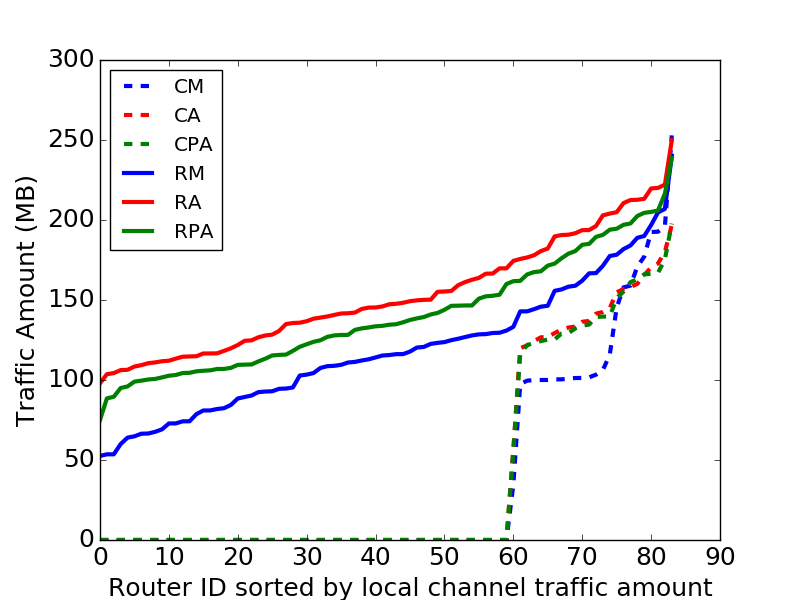
\includegraphics[height=1.5 in]{syn-wkld/cr/lc-traffic}
        \caption{CR Local Channel Traffic}
        \label{fig:syn-cr-lc-traffic}
    \end{subfigure}\\
    \centering
    \begin{subfigure}[t]{0.32\textwidth}
        \centering
        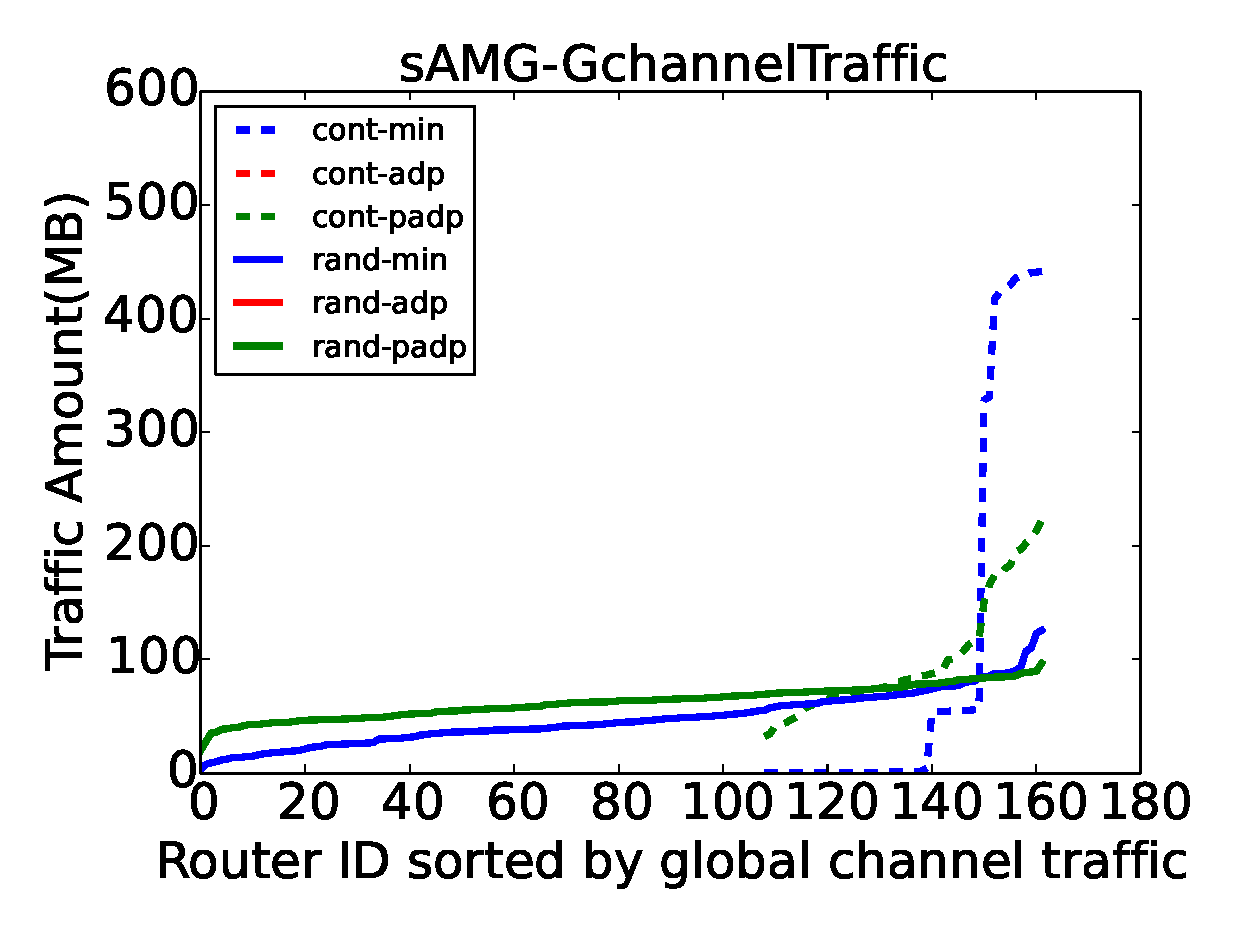
\includegraphics[height=1.5 in]{syn-wkld/amg10/gc-traffic}
        \caption{sAMG Global Channel Traffic}
        \label{fig:syn-samg-gc-traffic}
    \end{subfigure}\hfill
    \hspace{1em}%
    \begin{subfigure}[t]{0.32\textwidth}
        \centering
        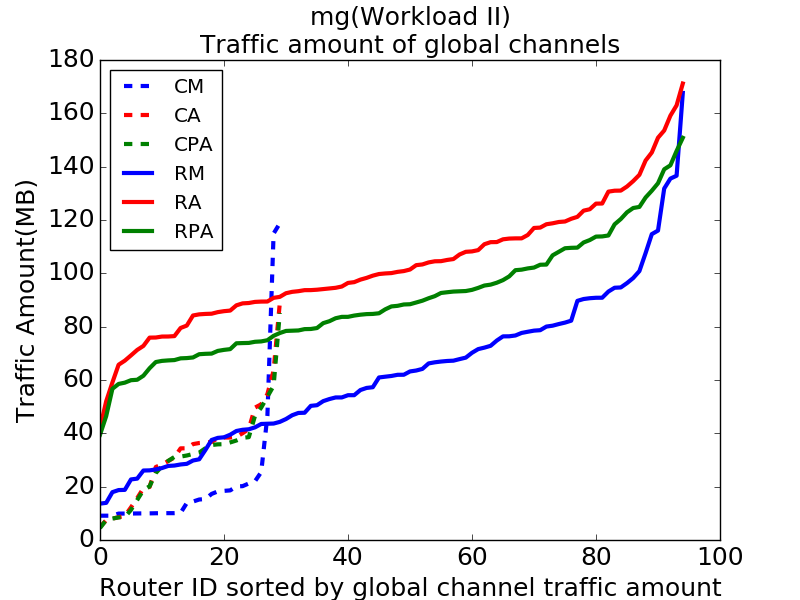
\includegraphics[height=1.5 in]{syn-wkld/mg/gc-traffic}
        \caption{MG Global Channel Traffic}
        \label{fig:syn-mg-gc-traffic}
    \end{subfigure}\hfill
    \begin{subfigure}[t]{0.32\textwidth}
        \centering
        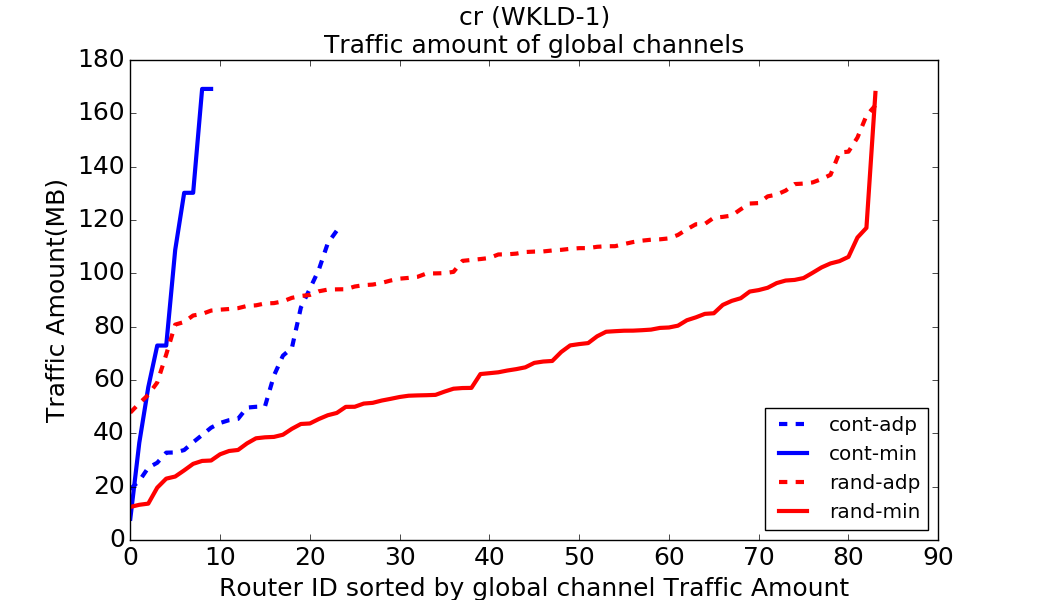
\includegraphics[height=1.5 in]{syn-wkld/cr/gc-traffic}
        \caption{CR Global Channel Traffic}
        \label{fig:syn-cr-gc-traffic}
    \end{subfigure}%
   \caption{The aggregate traffic go through the local and global channels of routers serving specific application. ``CA" and ``CPA" perform comparably, the corresponding lines are overlapped. More routers are involved in serving each application when random placement is in use, compared with contiguous placement.}
   \label{fig:syn-3app-gc-traffic}
\end{figure*}


\subsection{Key Observations}

In summary, based on the Workload \Rmnum{2}, we have made the following observations.

\emph{The application becomes ``bully" in the workload only because it has more amount of data transfer compared with its concurrently running peers.} ``Bully" application takes advantage of the network resource belonging to other applications when network sharing is enabled by random placement and adaptive routing policy. 


\emph{The communication-intensive is a relative metric between concurrently running jobs.} MultiGrid and CrystalRouter are the ``bully" in Workload \Rmnum{1} and they become the ``bullee" when running concurrently with sAMG in Workload \Rmnum{2}.


\section{Hybrid Job Placement}
\label{sec: hybrid placement}

The precaution to stop ``bully" behavior is to avoid network sharing between concurrently running jobs. Using contiguous placement and minimal routing could be a way to avoid network sharing, but network performance could suffer degradation due to local congestion. Running each job with dedicated routing policy is unrealistic, since routing policy is pre-configured and can not be changed on the fly upon job submission. However, the job placement policies can be versatile for assigning different allocation (contiguous or random) to specific application.

Thus, we propose the hybrid placement as a reconcile solution. In the hybrid placement, the less communication-intensive applications get contiguous allocation while the communication-intensive ones get random allocation. We evaluate the effect of hybrid placement on improving network performance as well as preserving the performance of individual application. In following experiments with Workload \Rmnum{1}, the hybrid placement policy assigns AMG with contiguous allocation, MultiGrid and CrystalRouter with random allocations. \footnote{Due to page limit, we won't present the analysis about network traffic and saturated time in this section.}

\subsection{Network Performance Analysis}

Hybrid placement is also coupled with three routing policies, Minimal, Adaptive and Progressive Adaptive. They are denoted respectively as HM, HA and HPA. As presented in the previous section, random placement outperforms contiguous placement in terms of network performance, we only compare the results of hybrid placement with random placement due to the page limit.


\begin{table}[ht]
\begin{center}
\caption{Average time spent on communication by all MPI ranks when Workload I is running on dragonfly network under hybrid placement and random placement policies.} 
\label{tab: hyb-placement-wkld-commtime}
\begin{tabular}{l c c c c c c }
\toprule % Top horizontal line
\toprule
&\multicolumn{6}{c}{Placement and Routing Configurations} \\
\cmidrule(l){2-7}
	      & HM & HA & HPA & RM & RA & RPA \\ % Column names row
\midrule % In-table horizontal line
Time(ms)  &273 &255 &255 &255 &265 &264  \\ % Content row 1
%\midrule
%Workload II &1747 &1991 &1991 &1791 &2367 &1965 \\
\midrule % In-table horizontal line
\bottomrule % Bottom horizontal line
\end{tabular}
\end{center}
\end{table}


As shown in Table \ref{tab: hyb-placement-wkld-commtime}, hybrid placement and random placement perform comparably. When coupled with minimal routing, RM outperforms HM. However, when coupled with (progressive) adaptive routing, HA and HPA outperform RA and RPA. HA and HPA perform equally well as compared with RM.  


\subsection{Individual Application Analysis}

\begin{figure*}[t!]
    \centering
    \begin{subfigure}[t]{0.32\textwidth}
        \centering
        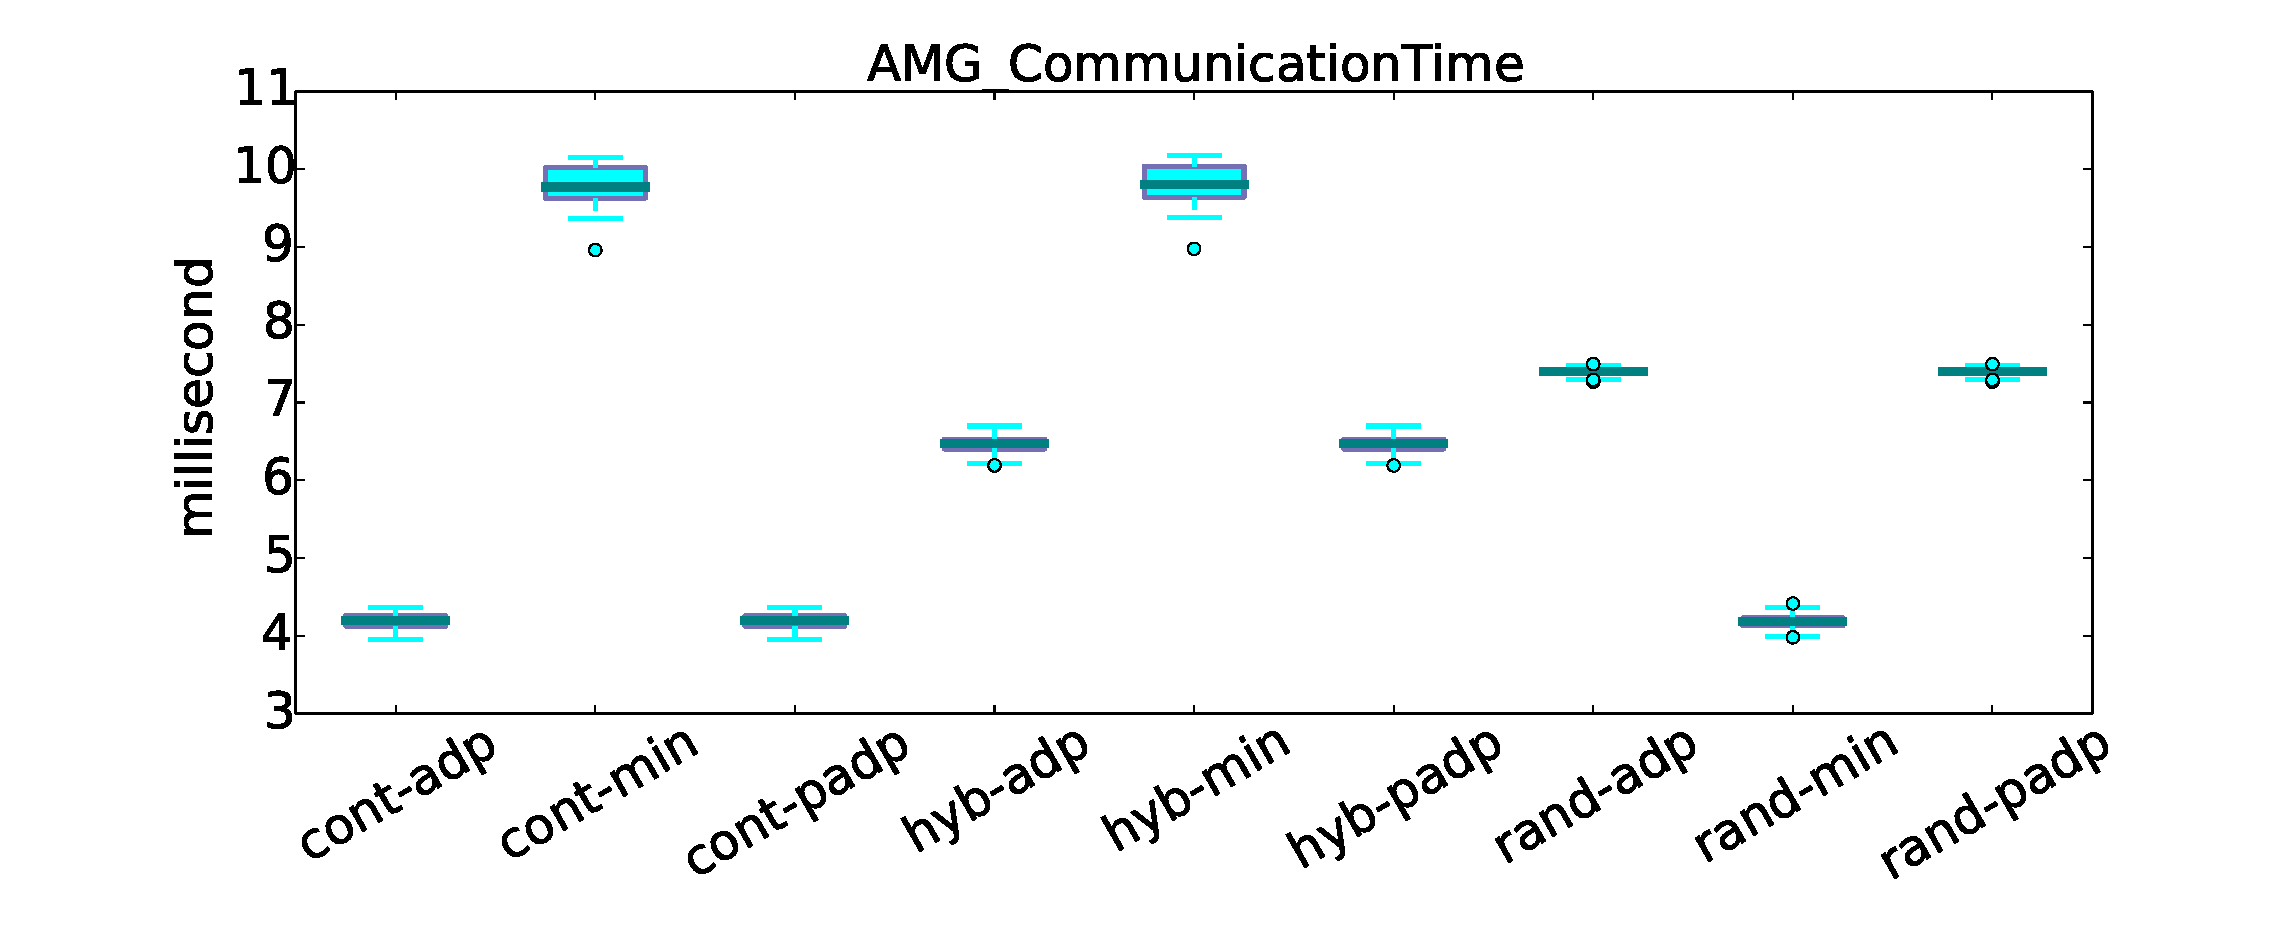
\includegraphics[height=1.3 in]{hyb-plcmt/amg/commtime}
        \caption{AMG Communication Time}
        \label{fig:hyb-plcmt-amg-commtime}
    \end{subfigure}\hfill
    \hspace{1em}%
    \begin{subfigure}[t]{0.32\textwidth}
        \centering
        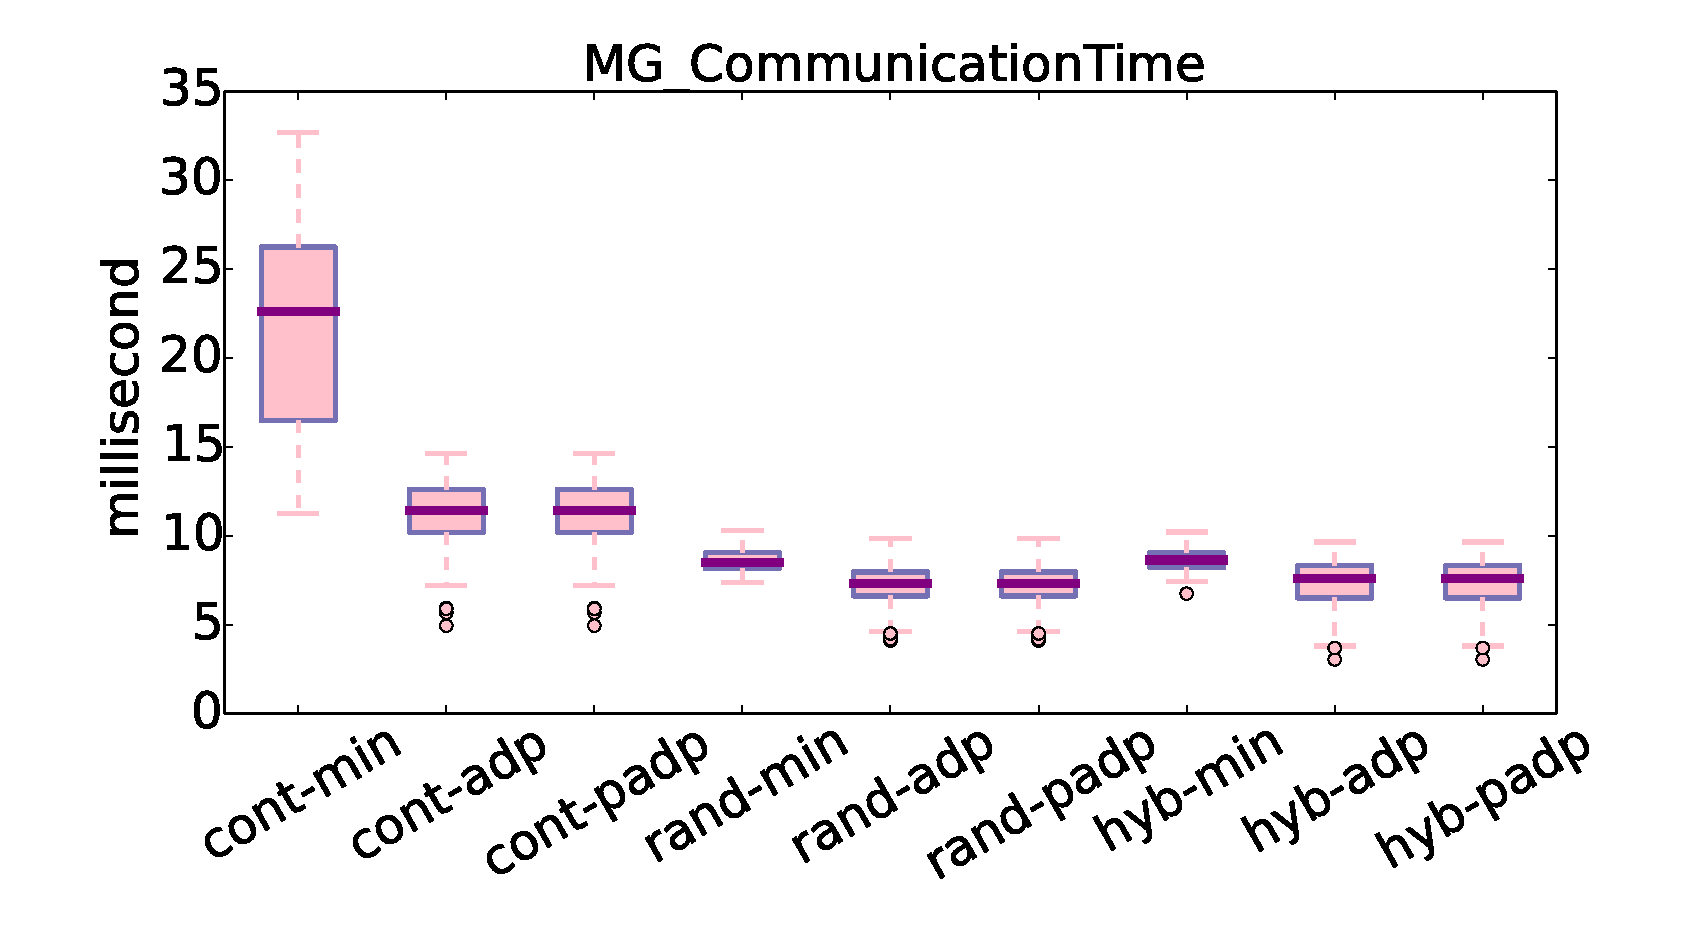
\includegraphics[height=1.3 in]{hyb-plcmt/mg/commtime}
        \caption{MG Communication Time}
        \label{fig:hyb-plcmt-mg-commtime}
    \end{subfigure}\hfill
    \begin{subfigure}[t]{0.32\textwidth}
        \centering
        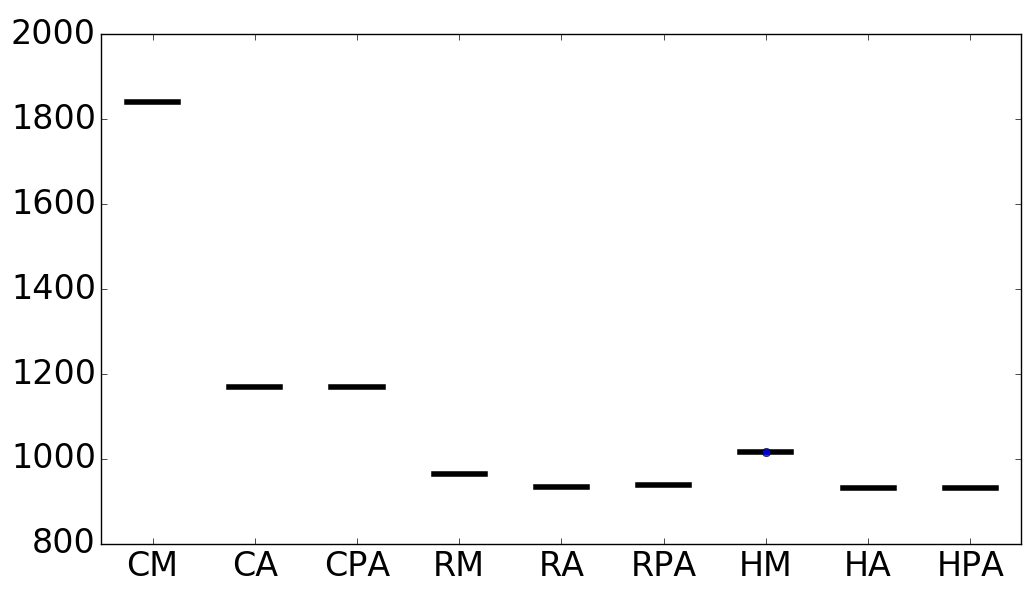
\includegraphics[height=1.3 in]{hyb-plcmt/cr/commtime}
        \caption{CR Communication Time}
        \label{fig:hyb-plcmt-cr-commtime}
    \end{subfigure}%
   \caption{Application communication time. Workload \Rmnum{1} is running under all the possible placement and routing configurations.}
   \label{fig:hyb-plcmt-apps-commtime}
\end{figure*}

Figure \ref{fig:hyb-plcmt-apps-commtime} shows the communication time of each application when hybrid placement configurations are in use. MultiGrid and CrystalRouter have basically the same performance with hybrid placement as compared with random placement. Since they still get random allocation in the hybrid placement. The performance of AMG is significantly improved when hybrid placement is in use. Compared with ``RA" and ``RPA", ``HA" and ``HPA" can greatly reduce AMG communication time, shown in Figure \ref{fig:hyb-plcmt-amg-commtime}. This is due the contiguous allocation assigned to AMG in the hybrid placement policy. When being coupled with minimal routing, hybrid placement and contiguous placement have similar performance for AMG. However, when (progressive) adaptive routing are in use, the traffic from MultiGrid and CrystalRouter still might be redirected to the routers serving AMG. Since AMG is less communication-intensive and can not fully utilize network, it is likely that the intermediate routers picked for the traffic from MultiGrid and CrystalRouter could be from AMG's groups. So for AMG, ``HA" and ``HPA" are worse than ``CA" and ``CPA", but they are much better than ``RA" and ``RPA".

\subsection{Key Observations}

Based on the results from experimenting with hybrid placement policy, we can make the following observations.

\emph{Compared with random placement policy, hybrid placement can guarantee comparable network performance.} Hybrid placement policy allows network sharing between communication intensive applications, thus alleviates the potential congestion and improves network utilization.

\emph{Hybrid placement can mitigate the performance degradation of less communication-intensive application.} Hybrid placement policy preserves contiguous allocation for less communication-intensive application, prevents network resource from being shared by others. Unlike random placement indulging the ``bully", hybrid placement can restrain it to some extent.

Hybrid placement can guarantee the performance of individual application without causing performance degradation to network performance. Compared with contiguous and random placement policy, hybrid placement are more preferable to HPC systems with dragonfly networks.


\section{Related Work}
\label{sec:related work}

The impact of job placement to both system and application always catches researchers' appetite \cite{dskinner} \cite{abhinav-sc13} \cite{jose-ipdps15}. Skinner et al. identified that network congestion could cause significant performance variability \cite{dskinner}. Bhatele et al. studied the performance variability of a specific application, p3FD, running on different production systems with torus networks \cite{abhinav-sc13}. They noticed that the application performance would keep consistent when it got compact allocation and exclusive network resource. Jokanovic et al. studied the impact of job placement to the workload and claimed that the key to reduce performance variability is to avoid network sharing \cite{jose-ipdps15}. 

Recently, several researchers have investigated the job placement and routing schemes on dragonfly network. Bogdan et al. proposed novel solution for mapping tasks of application that conforms to Nearest Neighbor communication pattern on dragonfly network \cite{hoefler-hpdc14}. Jain et al. conducted a comprehensive analysis of various job placement and routing policies with regard to network link throughput on dragonfly network \cite{jain-sc14}. Their work is based on an analytical model and synthetic workload. Bhatele et al. used simulation to study the performance of synthetic workload under the different task mapping and routing policies on two-level direct networks \cite{bhatele-sc11}.


Our work different from the previous works in the following ways. First, instead of using synthetic workload that generated based on predefined communication patterns, our simulation is driven by real application traces collected from production system. Second, not only we care about the workload performance, but also we pay attention to each individual application in the workload. We found that although random placement coupled with adaptive routing can improve the network performance, the less communication-intensive applications in the workload may suffer performance degradation. Third, with the sophisticated simulation tool CODES, we can not only get applications communication information, but also the insight about the network performance when application is running. The traffic and saturated time of router's each link are valuable information for detailed analysis.

\section{Conclusion}
\label{sec:conclusion}

In this paper, we have conducted extensive study about application's behavior when running on dragonfly network with different job placement and routing configurations. We resorted to CODES, a high-fidelity HPC network simulation tool, and used three parallel scientific applications traces collected from production system to analyze the applications' behavior on network level. We found that when applications are running concurrently, although random placement can uniformly distribute the workload traffic over the network to reach load balance and hot-spots free for the network, the performance of certain job would be impaired. We identify this phenomenon as ``bully" between concurrently running jobs, and the victim always being the less communication-intensive one. On the other hand, the contiguous placement tend to cause local congestion, however when coupled with adaptive routing, it can guarantee the performance of ``bullee" application by limiting the network sharing from concurrently running peers. 

Due the presence of this ``bully", we propose to use hybrid placement policy for workload running on systems with dragonfly networks. In hybrid placement policy, the less intensive applications get contiguous allocations, and the intensive ones get random allocations. We believe the findings presented in this paper can illuminate a path to more efficient workload manager for future systems with dragonfly network.



% conference papers do not normally have an appendix



% use section* for acknowledgment
\ifCLASSOPTIONcompsoc
  % The Computer Society usually uses the plural form
  \section*{Acknowledgments}
\else
  % regular IEEE prefers the singular form
%   \section*{Acknowledgment}
\fi


The work at Illinois Institute of Technology is supported in part by U.S. National Science Foundation grants CNS-1320125 and CCF-1422009. This work is also supported by the U.S. Department of Energy, Office of Science, Advanced Scientific Computing Research, under Contract DE-AC02-06CH11357.


% trigger a \newpage just before the given reference
% number - used to balance the columns on the last page
% adjust value as needed - may need to be readjusted if
% the document is modified later
%\IEEEtriggeratref{4}


\bibliographystyle{IEEEtran}
\bibliography{./reference}  


 \vspace{1\baselineskip}
 
 \begin{framed}
 The submitted manuscript has been created by UChicago Argonne, LLC, Operator of Argonne National Laboratory ("Argonne").  Argonne, a U.S. Department of Energy Office of Science laboratory, is operated under Contract No. DE-AC02-06CH11357.  The U.S. Government retains for itself, and others acting on its behalf, a paid-up nonexclusive, irrevocable worldwide license in said article to reproduce, prepare derivative works, distribute copies to the public, and perform publicly and display publicly, by or on behalf of the Government.
 \end{framed}


\end{document}


